%% 
%% Copyright 2019-2021 Elsevier Ltd
%% 
%% This file is part of the 'CAS Bundle'.
%% --------------------------------------
%% 
%% It may be distributed under the conditions of the LaTeX Project Public
%% License, either version 1.2 of this license or (at your option) any
%% later version.  The latest version of this license is in
%%    http://www.latex-project.org/lppl.txt
%% and version 1.2 or later is part of all distributions of LaTeX
%% version 1999/12/01 or later.
%% 
%% The list of all files belonging to the 'CAS Bundle' is
%% given in the file `manifest.txt'.
%% 
%% Template article for cas-sc documentclass for 
%% single column output.


\documentclass[a4paper,fleqn]{cas-sc}
% Use to make nonmenclature
\usepackage{framed} % Framing content
\usepackage{multicol} % Multiple columns environment
\usepackage{amsmath}
\usepackage{nomencl} % Nomenclature package
\usepackage{subcaption}
\usepackage{hyperref}
\usepackage[numbers]{natbib}

\makenomenclature

\renewcommand{\nomgroup}[1]{%
\ifthenelse{\equal{#1}{A}}{\item[\textbf{Variables}]}{%
\ifthenelse{\equal{#1}{C}}{\item[\textbf{Abbreviations}]}{%
\ifthenelse{\equal{#1}{B}}{\item[\textbf{Greek variables}]}{}}}
}
\setlength{\nomitemsep}{-\parskip} % Baseline skip between items
\renewcommand*\nompreamble{\begin{multicols}{2}}
\renewcommand*\nompostamble{\end{multicols}}
% If the frontmatter runs over more than one page
% use the longmktitle option.

%\documentclass[a4paper,fleqn,longmktitle]{cas-sc}
\addtolength{\jot}{3mm}
\usepackage[numbers]{natbib}
%\usepackage[authoryear]{natbib}
%\usepackage[authoryear,longnamesfirst]{natbib}

%%%Author macros
\def\tsc#1{\csdef{#1}{\textsc{\lowercase{#1}}\xspace}}
\tsc{WGM}
\tsc{QE}
%%%

\newcommand{\nomunit}[1]{%
   \renewcommand{\nomentryend}{\unskip\dotfill #1}}

% Uncomment and use as if needed
\newtheorem{theorem}{Algorithm}
\newtheorem{lemma}[theorem]{Lemma}
%\newdefinition{rmk}{Remark}
%\newproof{pf}{Proof}
%\newproof{pot}{Proof of Theorem \ref{thm}}

\begin{document}
\let\WriteBookmarks\relax
\def\floatpagepagefraction{1}
\def\textpagefraction{.001}

% Short title
\shorttitle{}    

\shortauthors{B.T. Rawlins et el.}  

% Main title of the paper
\title [mode = title]{An integrated data-driven surrogate model and thermofluid network-based model of a 620 $MW_e$ utility-scale boiler}  

% Title footnote mark
% eg: \tnotemark[1]
%\tnotemark[<tnote number>] 

% Title footnote 1.
% eg: \tnotetext[1]{Title footnote text}
%\tnotetext[<tnote number>]{<tnote text>} 

% First author
%
% Options: Use if required
%\author[1,3]{Author Name}[type=editor,
%       style=chinese,
%       auid=000,
%       bioid=1,
%       prefix=Sir,
%       orcid=0000-0000-0000-0000,
%       facebook=<facebook id>,
%       twitter=<twitter id>,
%       linkedin=<linkedin id>,
%       gplus=<gplus id>]

\author[1]{B.T. Rawlins}

% Corresponding author indication
\cormark[1]
\cortext[1]{Corresponding author}
% Footnote of the first author
%\fnmark[<footnote mark no>]

% Email id of the first author
\ead{rwlbra001@myuct.ac.za}

% URL of the first author
%\ead[url]{<URL>}

% Credit authorship
% eg: \credit{Conceptualization of this study, Methodology, Software}
\credit{Methodology, Software, Validation, Formal analysis, Investigation,Writing original draft, Visualization.}

% Address/affiliation
\affiliation[1]{organization={Department of Mechanical Engineering, Applied Thermal-Fluid Process Modelling Research Unit, University of Cape Town},
            addressline={Library Road, Rondebosch}, 
            city={Cape Town},
%          citysep={}, % Uncomment if no comma needed between city and postcode
            postcode={7701}, 
            %state={},
            country={South Africa}}

\author[2]{Ryno Laubscher}[]

% Footnote of the second author
%\fnmark[2]

% Email id of the second author
%\ead{rlaubscher@sun.ac.za}
% URL of the second author
%\ead[url]{}
% Credit authorship
\credit{Writing review \& editing, Methodology, Resources, Conceptualization.}
% Address/affiliation
\affiliation[2]{organization={Department of Mechanical Engineering, Stellenbosch University},
            addressline={Banghoek Road, Stellenbosch}, 
            %city={Stellenbosch},
%          citysep={}, % Uncomment if no comma needed between city and postcode
            postcode={7600}, 
            %state={},
            country={South Africa}}
% Footnote text
%\fntext[1]{}
% For a title note without a number/mark
%\nonumnote{}
\author[1]{Pieter Rousseau}
% Email id of the second author
%\ead{pieter.rousseau@uct.ac.za}
% Credit authorship
\credit{Writing review \& editing, Resources, Conceptualization}

% Corresponding author text

% Here goes the abstract
\begin{abstract}
An integrated data-driven surrogate model and one-dimensional (1D) process model of a 620 $MW_e$ utility scale boiler is presented. A robust and computationally inexpensive computational fluid dynamic (CFD) model of the utility boiler was utilized to generate the solution dataset for surrogate model training and testing. Both a standard multi-layer perceptron (MLP) and MLP connected mixture density network (MDN) machine learning architectures are compared for use as a surrogate model to predict the furnace heat loads and the flue gas inlet conditions to the convective pass. A hyperparameter search was performed to find the best MLP and MLP-MDN architecture. The MDN was selected for surrogate model integration since it showed comparable accuracy and provides the ability to predict the uncertainty in the results. Validation of the integrated model against plant data was performed for a wide range of loads and critical results were predicted within 5-8\% of the measured results. The validated model was subsequently used to investigate the effects of using a poor-quality fuel for the 100\% maximum continuous rating (MCR) load case. The uncertainties predicted by the surrogate model were propagated through the integrated model using the Monte Carlo technique, adding valuable insight into the operational limits of the power plant and the uncertainties associated with it. 
\end{abstract}

% Use if graphical abstract is present
%\begin{graphicalabstract}
%\includegraphics{}
%\end{graphicalabstract}

% Research highlights
\begin{highlights}
\item Data-driven surrogate model development using CFD solution data.
\item Development of mixture density network using simulation data.
\item Surrogate model integration with 1-D process model.
\item Off-design fuel quality investigation.
\end{highlights}

% Keywords
% Each keyword is seperated by \sep
\begin{keywords}
Mixture density network \sep Data-driven surrogate modelling \sep Computational fluid dynamics \sep Coupled simulation
\end{keywords}



\maketitle
% Main text
\section{Introduction}\label{intro}
A significant portion of the developing world still rely on conventional coal fired power plants to meet local energy demands \cite{Rousseau2020}. However, increased penetration of renewable energy sources onto electrical grids will force conventional base-load thermal power plants to operate on a mid-merit basis. Mid-merit operation requires improved flexibility with faster load following characteristics and start-up rates \cite{Safdarnejad2019}, as well as running at off-design and low load conditions for extended periods. This can result in an increase in thermal stresses on key operational components \cite{Modlinski2019}. Therefore, it is important to be able to predict the integrated thermofluid response of boilers and the impact on components at off-design conditions. Computational fluid dynamic (CFD) models are typically utilised in modelling the fire-side interactions of pulverised coal fired boilers \cite{}, since the modelling approach can adequately resolve the complex fluid flow and heat transfer phenomena, including the mechanical and thermal interactions between the flue gas and the particles. CFD simulations are predominately used for detailed exploration of the flue gas side flow and heat transfer phenomena of boilers to investigate pollutant production \cite{Liu2021}, perform design optimization \cite{dugum2019, Gu2020} and study particle effects \cite{Laubscher2020}. For utility-scale boilers the associated computational burden practically limits the use of CFD to steady-state analysis of specific areas of interest, such as the furnace and radiant heat exchangers, and does not allow for integrated whole-boiler modelling in other words modelling the water- and flue gas-sides in a single model.\\
\begin{table*}[!t]   
\begin{framed}
\nomenclature[C]{$CFD$}{Computational Fluid Dynamics}
\nomenclature[C]{$HHV$}{Higher Heating Value}
\nomenclature[C]{$ROM$}{Reduced Order Model}
\nomenclature[C]{$ANN$}{Artificial Neural Network}
\nomenclature[C]{$DOE$}{Design of Experiments}
\nomenclature[C]{$EDM$}{Eddy Dissipation Model}
\nomenclature[C]{$MDN$}{Mixture Density Network}
\nomenclature[C]{$ATT$-$RH$}{Reheater Attemperator}
\nomenclature[C]{$ATT2$}{Attemperator 1}
\nomenclature[C]{$ATT1$}{Attemperator 2}
\nomenclature[C]{$J_{MSE}$}{Mean Square Error cost function}
\nomenclature[C]{$J_{NLL}$}{Negative Log Likelihood cost function}
\nomenclature[C]{$RMSE$}{Root Mean Square}
\nomenclature[C]{$RNN$}{Recurrent Neural Network}
\nomenclature[C]{$MLP$}{Multi-layer Perceptron}
\nomenclature[C]{$MAE$}{Mean Absolute Error}
\nomenclature[C]{$MSE$}{Mean Square Error}
\nomenclature[C]{$SH2$}{Platen Superheater}
\nomenclature[C]{$SH1$}{Primary Superheater}
\nomenclature[C]{$SH3$}{Final Superheater}
\nomenclature[C]{$RH1$}{Primary Reheater}
\nomenclature[C]{$RH2$}{Secondary Reheater}
\nomenclature[C]{$EC$}{Economiser}
\nomenclature[C]{$EV$}{Evaporator}
\nomenclature[A]{$u$}{Directional velocity \nomunit{$m/s$}}
\nomenclature[A]{$\bar{P}_r$}{Surrogate model prediction vector \nomunit{$-$}}
\nomenclature[B]{$\bar{\mu}_k$}{MDN predicted mean for distribution $k$ \nomunit{$-$}}
\nomenclature[B]{$\bar{\theta}_k$}{MDN standard deviation for distribution $k$ \nomunit{$-$}}
\nomenclature[B]{$\bar{\pi}_k$}{MDN mixing coefficient for distribution $k$ \nomunit{$-$}}
\nomenclature[A]{$\bar{Y}$}{CFD solution output vector \nomunit{$-$}}
\nomenclature[A]{$\bar{X}$}{High-level input vector \nomunit{$-$}}
\nomenclature[A]{$p$}{Pressure \nomunit{$Pa$}}
\nomenclature[A]{$p_{O_2}$}{Oxygen partial pressure \nomunit{$Pa$}}
\nomenclature[A]{$P$}{Perimeter \nomunit{$m$}}
\nomenclature[A]{$R_{vol}$}{Volatile reaction rate \nomunit{$s^{-1}$}}
\nomenclature[A]{$R_{c}$}{Chemical reaction rate \nomunit{$kg/m^2 sPa$}}
\nomenclature[A]{$R_{diff}$}{Diffusion reaction rate coefficient \nomunit{$kg/m^2 sPa$}}
\nomenclature[A]{$A_{vol}$}{Volatile pre-exponential factor \nomunit{$s^{-1}$}}
\nomenclature[A]{$A_{c}$}{Char pre-exponential factor \nomunit{$kg/m^2sPa$}}
\nomenclature[A]{$A$}{Area \nomunit{$m^{2}$}}
\nomenclature[A]{$E_{a,c}$}{Char activation energy \nomunit{$J/mol$}}
\nomenclature[A]{$E_{a,vol}$}{Volatile matter activation energy  \nomunit{$J/mol$}}
\nomenclature[A]{$m_{c}$}{Char mass \nomunit{$kg$}}
\nomenclature[A]{$m_{b}$}{Batch size \nomunit{$-$}}
\nomenclature[A]{$\bar{h}_{l}$}{Neural network signal for layer $l$ \nomunit{$-$}}
\nomenclature[A]{$\bar{z}_{l}$}{Summed signal to network neural for layer $l$ \nomunit{$-$}}
\nomenclature[A]{$d_{p}$}{Particle diameter \nomunit{$m$}}
\nomenclature[A]{$m_{c}$}{Volatile mass \nomunit{$kg$}}
\nomenclature[A]{$E$}{Total energy \nomunit{$J/kg$}}
\nomenclature[A]{$Y_k$}{Mass fraction of species $k$ \nomunit{$kg/kg$}}
\nomenclature[A]{$T_g$}{Gas temperature \nomunit{$K$}}
\nomenclature[A]{$T_p$}{Particle temperature \nomunit{$K$}}
\nomenclature[B]{$\lambda$}{Thermal conductivity \nomunit{$W/mK$}}
\nomenclature[B]{$\mu$}{Viscosity \nomunit{$Pa.s$}}
\nomenclature[A]{$S$}{Mass source term \nomunit{$kg/m^3$}}
\nomenclature[A]{$S_m$}{Momentum source term \nomunit{$N/m^3$}}
\nomenclature[A]{$S_h$}{Energy source term\nomunit{$W/m^3$}}
\nomenclature[A]{$S_k$}{Species source term \nomunit{$kg/m^3$}}
\nomenclature[A]{$J_k$}{Diffusion flux of species $k$ \nomunit{$kg/m^3$}}
\nomenclature[B]{$\rho$}{Gas density \nomunit{$kg/m^3$}}
\nomenclature[B]{$\rho_{eff}$}{Effective density \nomunit{$kg/m^3$}}
\nomenclature[B]{$\rho_{M}$}{Mixture density \nomunit{$kg/m^3$}}
\nomenclature[B]{$\rho_{l}$}{Liquid phase density \nomunit{$kg/m^3$}}
\nomenclature[A]{$h_{M}$}{Mixture enthalpy \nomunit{$J/kg$}}
\nomenclature[A]{$x$}{Quality \nomunit{$-$}}
\nomenclature[B]{$\rho_{g}$}{Gas phase density \nomunit{$kg/m^3$}}
\nomenclature[B]{$\eta$}{Learning rate \nomunit{$-$}}
\nomenclature[B]{$\alpha_{M}$}{Mixture fraction \nomunit{$-$}}
\nomenclature[B]{$\phi_{mp}$}{Pseudo particle mass fraction \nomunit{$kg/kg_{fuel}$}}

\printnomenclature
\end{framed}
\end{table*}

Investigating the integrated whole-boiler thermofluid response requires the use of 1-D process models to capture the response of the steam/water cycle integrated with suitable models of the flue gas side in a co-simulation approach. Rousseau and Laubscher \cite{Rousseau2020} used this approach, utilising a 1-D process model of the water-side and CFD model of the fire-side, to investigate the effects high ash fuel has on the heat absorption of the radiant superheaters (SHs). As expected, this requires significant computational resources on the CFD side to allow for the integration of the two different models and is therefore not a feasible approach for extensive studies of flexible operation. This has led to the development of reduced order multiphase modelling approaches \cite{Rawlins2021, INFUB2022}, which proved to reduce the computational effort by approximately 25\% for a full-scale utility boiler.  However, this is still not enough to allow direct integration of CFD into whole-boiler system analysis tools which cannot be used to quickly analyse different operating cases.\\

Data-driven surrogate models can potentially be used to reduce the computational burden introduced via the CFD model. Data driven surrogate models form part of statistical regression models, where the predicted objective function is fitted using true evaluations of the objective function \cite{Wheeler2019}. Artificial neural networks (ANNs) are one of the most popular machine learning algorithms/techniques to facilitate the learning process. Other procedures include Kriging models \cite{Fei2015}, gradient boosting models \cite{Si2020,Qin2022} and support vector machines \cite{Lv2017}.\\

The works of Singh and Abbassi \cite{Singh2018} incorporated the use of an ANN and CFD model to investigate the transient thermal modelling of an off-highway machinery cabin. The ANN training data was obtained from a 1-D process model for the refrigeration cycle. The methodology was used successfully to integrate the ANN capabilities with a 3-D CFD simulation model thereby negating the need for a coupled simulation procedure. Similarly, Fei et al \cite{Fei2015} made use of a fast set of reduced order models (ROMs), using the Kriging method, based on CFD data to investigate the retrofitting of a coal fired power plant under oxy-fuel conditions. Using an integrated ROM with a process model, a range of air-coal conditions were investigated, with the model illustrating sufficiently accurate results. However, no operational uncertainty was incorporated into the input parameters to account for real world operational effects (disturbances, local atmospheric conditions etc.).\\

Acknowledging and predicting the impact of uncertainties in conventional coal fired power plants are paramount for the safe operation and maintenance of these plants \cite{Madejski_18}. The uncertainties associated with the operational parameters of thermal power plants, such as fuel quality, combustion processes, and  burner biasing, can lead to significant changes in the thermofluid response \cite{Sarkar2015}. The design space load uncertainty of a combined cooling, heating and power system was investigated by Lu et al \cite{Lu2021}. Using a multi-objective optimization model, factors such as pollutant emission, economy and the system reliability were incorporated to improve the operational performance. The model illustrated its future use for designers in providing the best configuration scheme under system load uncertainties.\\ 

It is noted that CFD cannot meet the near real time requirement for on-line performance monitoring, due to the complex solution mechanisms and time-consuming calculations. However, it is a feasible alternative to generate training and testing datasets for ANN implementation, since using CFD does not interfere with normal operation of the plant. In addition, a wider range of appropriate operating conditions can be simulated. The works of Shi et al. \cite{Shi2019} developed an optimisation method, which employed an ANN to predict the thermal efficiency and emission properties, for a 660 [$MW_e$] ultra-supercritical coal fired power plant. Training and testing data was obtained from historical operating data, as well as using the solution data of a 100 unique CFD simulation cases covering a wide range of operating cases. The additional CFD simulation data strengthened the generalization of the ANN model, mainly because the CFD simulation provided different kinds of operating condition making the model adapt to different working conditions. Good agreement between the predictions and measured data was realised with a maximum mean error of 0.04\%. Researchers Dal Secco et al. \cite{DalSecco2015}, conducted a comparable study to identify boiler operational configurations to minimise the $NO_x$ emissions in a 600 [$MW$] tangentially fired pulverised coal boiler. The study made use of a genetic algorithm to correlate the operating parameters to the output data produced from a large CFD simulation dataset. The genetic algorithm helped identify the optimal firing configurations from the CFD dataset that establish a good compromise between low $NO_x$ emissions and the reduction of fire-side corrosion.\\

In the present work, a modelling methodology is employed that incorporates the use of a CFD generated solution database in the training and testing of data-driven surrogate model that captures the fire-side of a 620 [$MW_e$] utility scale boiler. Subsequently, the data-driven surrogate model is integrated with a 1-D process model of the water-/steam-side. This integrated model is proposed to investigate the thermal response of the 620 [$MW_e$] utility scale boiler under investigation. An existing validated steady-state multiphase CFD model \cite{Rawlins2021, INFUB2022} was used to generate a CFD simulation dataset for 180 different operating states. To determine the required complexity of the data-driven surrogate model, two different ANN frameworks were considered, namely a standard multi-layer perceptron (MLP) and a mixture density network MDN, where the latter allows the introduction of uncertainty into the model predictions. A hyper-parameter search was conducted to establish the best performing model, with the lowest mean absolute error (MAE) being the essential criterion. Validation of the integrated model was performed for maximum continuous ratings (MCR) of 100\%, 80\% and 60\% load for which measured data is available. Following this, the validated model was used to investigate the impact of poor fuel quality at 100\% MCR, where the ash and moisture contents were varied for two separate cases.
\newpage
\section{Materials and methods}
The following section provides an overview of the case study boiler, the CFD modelling methodology utilised for the generation of testing and training data, the 1-D process model, and a description of the integrated model.
\subsection{Case study boiler}
The overall layout of the case study boiler is shown schematically in Figure \ref{fig_case_layout} \cite{Rousseau2020}. The boiler is defined as a two-pass sub-critical boiler, which is designed to deliver steam at a pressure of 16 [$MPa$] and an exit temperature of 535 [$^\circ C$] at full load. 
\begin{figure}[h!]
	\centering
		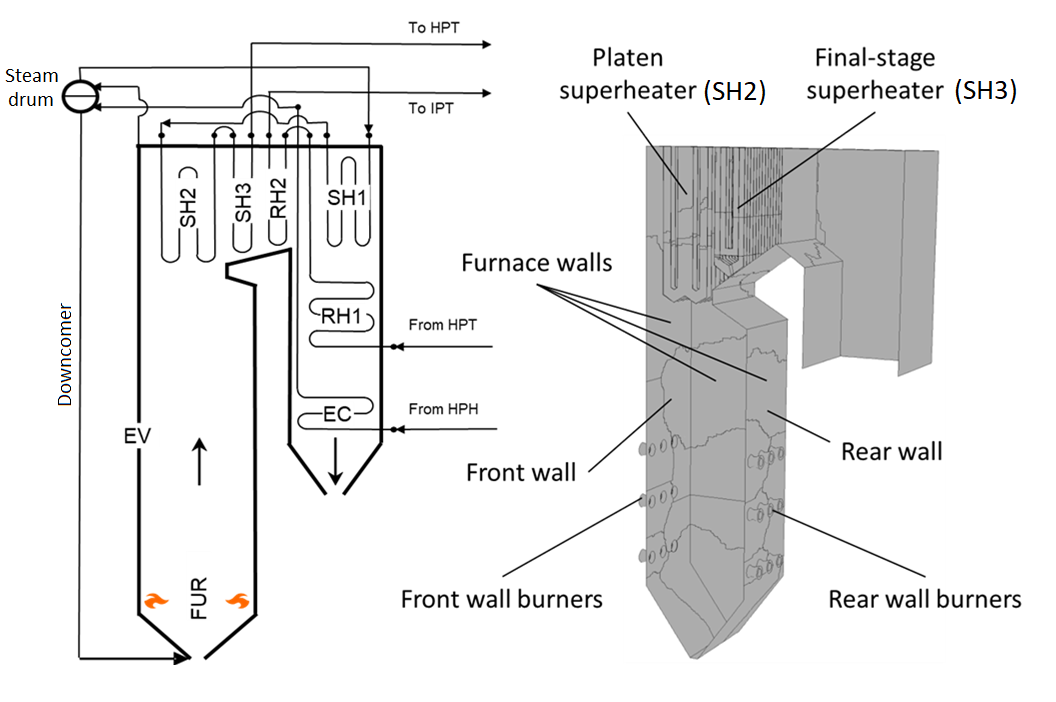
\includegraphics[scale=0.5]{CASE_STUDY_BOILER}
	  \caption{Case study boiler layout \citep{Rousseau2020}.}\label{fig_case_layout}
\end{figure}

The boiler forms part of a 620 [$MW_e$] power plant and consists of a furnace with water wall evaporator (EV), primary superheater (SH1), platen superheater (SH2) and final superheater (SH3), as well as a primary reheater (RH1), secondary reheater (RH2) and economiser (EC). The furnace height, width and depth are 64.0 [$m$], 24.0 [$m$], and 13.7 [$m$] respectively. The boiler furnace is fed by six mills, each supplying a pulverised fuel and primary air (PA) mixture to a burner row consisting of six opposing wall-mounted swirl burners. The fuel and PA mixture is injected through the inner annulus of the burner while the SA air is fed through the outer annulus as indicated in Figure \ref{fig_cfd_geom_bc}.

\subsection{CFD model}\label{sec_cfd}
The current study makes use of an existing steady-state multiphase CFD model \cite{INFUB2022}. The CFD model utilises an Eulerian-Eulerian approach to capture the solid and gaseous phase interactions. The model was implemented in the commercial CFD software package ANSYS Fluent\textsuperscript{\textregistered} v19.5 to resolve the fluid flow, heat transfer and combustion processes. The primary features of developed multiphase CFD model is the solution of two energy equations, one for the gas phase and another for the solid phase. This approach allows for the adequate resolution of the temperature-dependent combustion processes and accurate prediction of the particulate radiative effects. The model has been validated and verified for a 2.165 [$MW_{th}$] lab scale pulverised fuel burner by Rawlins et al. \cite{INFUB2022}. Furthermore, the CFD model was subsequently validated for the full-scale utility boiler of the current study operating for a wide range of loads \cite{Rawlins2021}. Thus, this section provides a summary of the CFD models features and governing equations.\\
\newpage
The CFD computational domain was created for half of the furnace width with a symmetry boundary condition located at 12.01 [$m$]. This was done to reduce the total cell count of the numerical mesh. Figure \ref{fig_cfd_geom_bc} highlights the computational domain and boiler geometry.\\
\begin{figure}[h!]
	\centering
		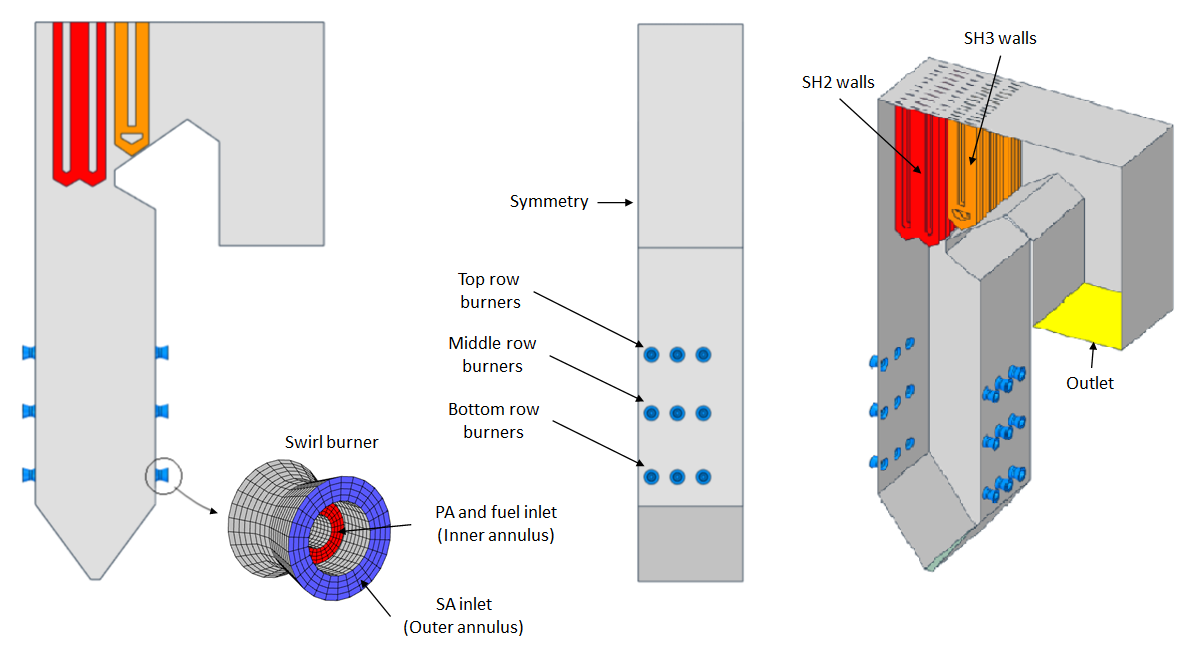
\includegraphics[scale=0.5]{CFD_GEOMETRY}
	  \caption{Overview of CFD model geometry and the computational domain.}\label{fig_cfd_geom_bc}
\end{figure}

The general conservation equations of mass, momentum, energy, and species were solved using an Eulerian approach. These are provided in Table \ref{tbl_govern}.
\begin{table}[pos = h]
\centering
\caption{Summary of CFD models governing equations}\label{tbl_govern}
\begin{tabular*}{0.8\textwidth}{p{0.2\textwidth}p{0.6\textwidth}}
\toprule
Conservation entity & Conservation equation\\
\midrule
Mass & $\frac{\partial}{\partial x_{i}}(\rho \bar{u}_{i})=S$\\[10pt]
Momentum& $\frac{\partial}{\partial x_{i}}(\rho_{eff} u_{i}u_{j})+\frac{\partial \overline{p}}{\partial x_{j}} = \frac{\partial}{\partial x_{i}}\left[\mu\left\{\frac{\partial u_{j}}{\partial x_{i}}+\frac{\partial u_{i}}{\partial x_{j}}-\frac{2}{3}\delta_{ij}\frac{\partial u_{i}}{\partial x_{i}}\right\}\right]+\frac{\partial}{\partial x_{i}}(-\rho\overline{u_{i}^{'}u_{j}^{'}})+S_m$\\[10pt]
Energy& $\frac{\partial }{\partial x_{i}} (u_{i}[\rho E+p])=\frac{\partial }{\partial x_{j}}\left[\lambda\frac{\partial T_{g}}{\partial x_{j}}\right] +S_{h}$\\[10pt]
Species&$\frac{\partial}{\partial x_{i}}(\rho u_{j}Y_{k})=-\frac{\partial}{\partial x_{j}}(\vec{J_{k}})+ \sum_r R_{j,r} + S_{k} \nonumber$\\
\bottomrule
\end{tabular*}
\end{table}


To account for the inertial effects the particles exert on the gas phase, an effective density ($\rho_{eff}$) was defined as follows:
\begin{equation}
\rho_{eff} = \frac{\rho \rho_{p}(\phi_{mp +1})}{\rho\phi_{mp}+\rho_p}
\end{equation}
where $\rho$, $\rho_p$ and $\phi_{mp}$ are the gas density, particulate density and the mass fraction of the pseudo particles present in a cell [$kg/kg_{fuel}$].\\

The solution of the Reynolds stress term found in the momentum equation ($-\rho\overline{u_{i}^{'}u_{j}^{'}}$) was approximated using the Boussineq equation \citep{Versteeg2007}. In the present study the realizable k-$\varepsilon$ turbulence model was utilized to address the turbulence closure problem and was selected for its applicability in modelling the effects of coal-fired swirl burners \citep{Modlinski2010}. The particle transport was modelled using general scalar transport equations of the pseudo-particle mass concentrations. The particulate scalar fields define the injected fuel based on the proximate fuel composition, namely the moisture, volatile matter, fixed carbon, and ash content.\\

The P-1 radiation model was used to resolve the radiative field in the domain. User-defined sources and functions were used to configure the Eulerian representation of the particle laden flow P-1 transport equation. In addition, the particles emissivity and scattering factor were modelled using variable correlations as applied by Lockwood et al. \cite{Lockwood1986} and Yin \cite{Yin2015}, respectively. Modelling of combustion follows a four-step sequential process, beginning with the heating and evaporation of the moisture present in the fuel, followed by the devolatilisation process where the volatiles are liberated from the solid particle, followed by the phenomena of char burnout, and finally the gas phase reactions would commence. The char oxidation reaction product species was set to that of carbon monoxide ($CO$). For the gas-phase reactions the turbulence-chemistry interaction was approximated using the eddy dissipation model (EDM). A summary of the combustion equations and constants are provided in Table \ref{tbl_combust}.
\begin{table}[pos = h]
\caption{Summary of combustion models and constants used in the CFD model}\label{tbl_combust}
\begin{tabular*}{\tblwidth}{p{0.325\textwidth}p{0.35\textwidth}p{0.25\textwidth}}
\toprule
Model & Equation/s & Constant/s\\
\midrule
\multicolumn{3}{l}{\textit{Devolatilization}} \\ % Table header row
Single rate kinetic model &$\frac{dm_{vol}}{dt} = R_{vol}(m_{0,vol}-m_{vol})$,  & $A_{vol} = 2\times10^5 [s^{-1}]$, \\
& $R_{vol} = A_{vol}exp\left(\frac{E_{a,vol}}{RT_p}\right)$ & $ E_{a,vol} = 6.7\times10^7 [J/mol]$ - \cite{Sheng2004} \\
\multicolumn{3}{l}{\textit{Char oxidation}} \\
Diffusion/kinetic - \citep{Baum1971} & $\frac{dm_{char}}{dt} = -A_p p_{O_{2}} \frac{R_{diff}R_c}{R_{diff} + R_c}$,  & $A_{c} = 0.0053 [kg/m^2sPa]$, \\
& $R_{c} = A_{c}exp\left(\frac{E_{a,c}}{RT_p}\right)$,  & $E_{a,c} = 8.37\times10^7 [J/mol]$ - \cite{Sheng2004} \\
& $R_{diff} = \frac{5\times10^{-12}}{d_p} \left(\frac{T_g+T_p}{2}\right)^{0.75}$&\\
\multicolumn{3}{l}{\textit{Gaseous reactions of volatiles and $CO$}} \\
Eddy dissipation model - \cite{Ansys} & $R_{k,r,P} =\vartheta_{k,r}M_{w,k}AB\rho\frac{\varepsilon}{k}min\left(\frac{\sum_{p} Y_p}{\sum_{j}\vartheta_{j,r}M_{w,j}}\right)$, $R_{k,r,R} =\vartheta_{k,r}M_{w,k}A\rho\frac{\varepsilon}{k}min\left(\frac{Y_R}{\vartheta_{R,r}M_{w,R}}\right)$ & $A=4.0$, $B=0.5$\\
\bottomrule
\end{tabular*}
\end{table}

The interested reader is directed to the works of Rawlins et al. \cite{Rawlins2021, INFUB2022, Rawlins2022} for a more detailed description of the developed CFD multiphase modelling approach.\\ 

To ensure that the results are grid independent, simulations were performed for mesh sizes of 3.5 million, 6 million and 10 million cells. The numerical mesh consisting of approximately 6 million cells was selected as the most efficient grid and was subsequently used for all the CFD simulations for generating the CFD solution data needed for the training and testing of the surrogate model. To ensure numerical stability during the simulation runs, the aspect ratio and mesh orthogonality quality were kept below 20 and above 0.2, respectively. The simulations were solved using the SIMPLE pressure–velocity coupling scheme. The pressure term was discretised using the PRESTO! scheme. Momentum, species, and energy equations were discretised using the second order upwind scheme and the turbulent kinetic energy and dissipation rate using the first-order upwind scheme. The convergence criteria for the simulation model were set to $1\times10^{-3}$ for the continuity equation, $1\times10^{-4}$ for the velocity monitors, $1\times10^{-6}$ for the remaining transport equations, and $1\times10^{-4}$ for monitored key parameters. Convergence criteria was enforced for all the various simulation runs.
\newpage
\subsection{Process model}\label{sec_process}
A 1-D discretised model of the furnace evaporator (EV), SH2, SH3, and subsequent downstream heat exchangers was developed using FlownexSE\textsuperscript{\textregistered} 2021 \cite{flownex}. The software can solve both the steady state and transient forms of the fundamental conservation equations of mass, energy, and momentum together with built in fluid property relations and component characteristics representative of all the different types of components. It is also possible to add control elements to obtain a complete integrated dynamic system simulation model of a plant, sub system or component.\\

The homogeneous two-phase mixture approach was used in modelling the heat exchanger water-side components of the entire boiler, whereby the fluid properties, phase velocities and temperatures are uniform per cross-sectional area. Table \ref{tbl_1dgovern} provides a summary 1-D models homogeneous property equations and governing transport equations.
\begin{table}[pos = h]
\caption{Summary of 1-D process models properties and governing equations}\label{tbl_1dgovern}
\begin{tabular*}{0.9\textwidth}{p{0.2\textwidth}p{0.75\textwidth}}
\toprule
Mixture property&Equation\\
\midrule
Mixture fraction&$\alpha_H = \frac{\rho_l x}{\rho_lx + \rho_g(1-x)}$ \\[10pt]
Mixture density& $\rho_M = (1-\alpha_H)\rho_l + \alpha_H\rho_g$\\
\midrule
Conservation entity & Conservation equation\\
\midrule
Mass & $\frac{\partial}{\partial t}(\rho_M A)+\frac{\partial}{\partial s}(\rho_MAu) = 0$\\[10pt]
Momentum& $\frac{1}{A} \frac{\partial}{\partial t}(\rho_M A u)+\frac{1}{A} \frac{\partial}{\partial s}(\rho_M A u^2) = -\frac{\partial p}{\partial s}-\frac{\tau_W P}{A}- \rho_M g \frac{\partial z}{\partial s}$\\[10pt]
Energy& $\frac{\partial}{\partial t}(\rho_Mh_M)+\frac{1}{A}\frac{\partial}{\partial s}(\rho_MAuh_M)+\frac{1}{2}\frac{\partial}{\partial s}(\rho_Mu^2)+
\frac{1}{2A}\frac{\partial}{\partial s}(\rho_MAu^3)=\frac{\partial p}{\partial t} + \frac{\dot{Q}_w}{V}-g\rho_Mu\frac{\partial z}{\partial s}$\\
\bottomrule
\end{tabular*}
\end{table}

The process model includes all the heat exchangers up to and downstream
of SH3, which includes heat exchangers RH2, SH1, RH1 and the EC. In addition, the model includes all the relevant attemperators (ATT1, ATT2, and ATT-RH), inlets, and outlets (refer to Figure \ref{fig_int_model}). The process model is used to determine the required attemperation flow rates and the overall water-/steam-side thermal response. The furnace EV, SH2 and SH3 walls are represented by single lumped pipe flow components.\\
\begin{figure}[h!]
\centerline{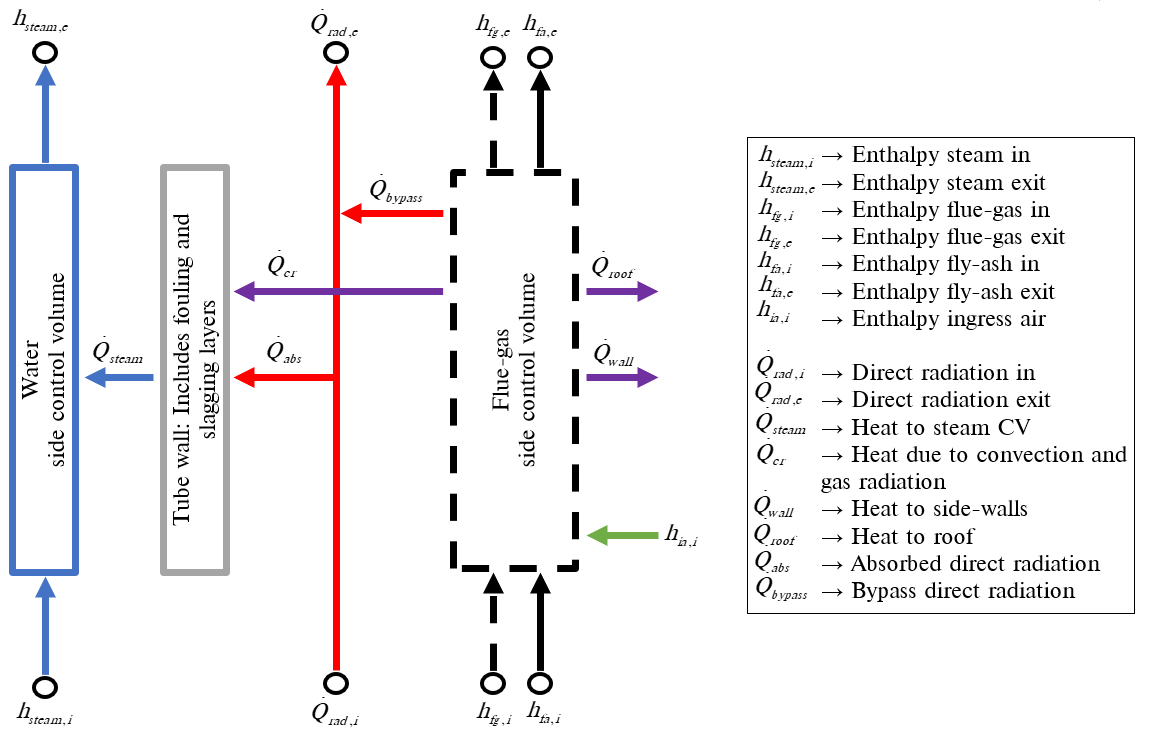
\includegraphics[scale=0.4]{HEAT_EXCHANGER_PROCESS_MODEL}}
\caption{Heat exchanger component model \cite{Rawlins2022}}
\label{fig_heatexh_model}
\end{figure}

The heat exchanger downstream of SH3 are modelled using a heat exchanger process model, which has successfully utilised in the works of Rawlins et al. \cite{Rawlins2022}. Figure \ref{fig_heatexh_model} illustrates the utilised heat exchanger process model. The component accounts for the radiative (gas and
direct), convective, and conduction heat transfer mechanisms to
and from the flue gas-side and water-/steam-side control volumes. The
total heat transferred to the water-/steam-side control volume can be
written as the sum of the absorbed direct radiation and the combined
convective and gas radiative heat transfer
\subsection{Integrated model}\label{sec_int_model}
The integrated model is primarily the integration of a data-driven surrogate model and a 1-D process model. The process model is used to capture the thermodynamic response of the water/steam side of the utility boiler under investigation, with the developed data-driven surrogate model providing predictions of the gas-side thermal characteristics (i.e., combustion product species, temperature, and incident radiation flux) and heat-exchanger heat loads to the EV, SH2 and SH3 walls. In the current study the development of the surrogate model follows two steps, namely data generation, utilising the CFD model presented in Section \ref{sec_cfd} to generate a training/testing dataset, and secondly the selection of the best machine learning model, based on the results of a hyperparameter search.\\ 
\begin{figure}[h!]
\centerline{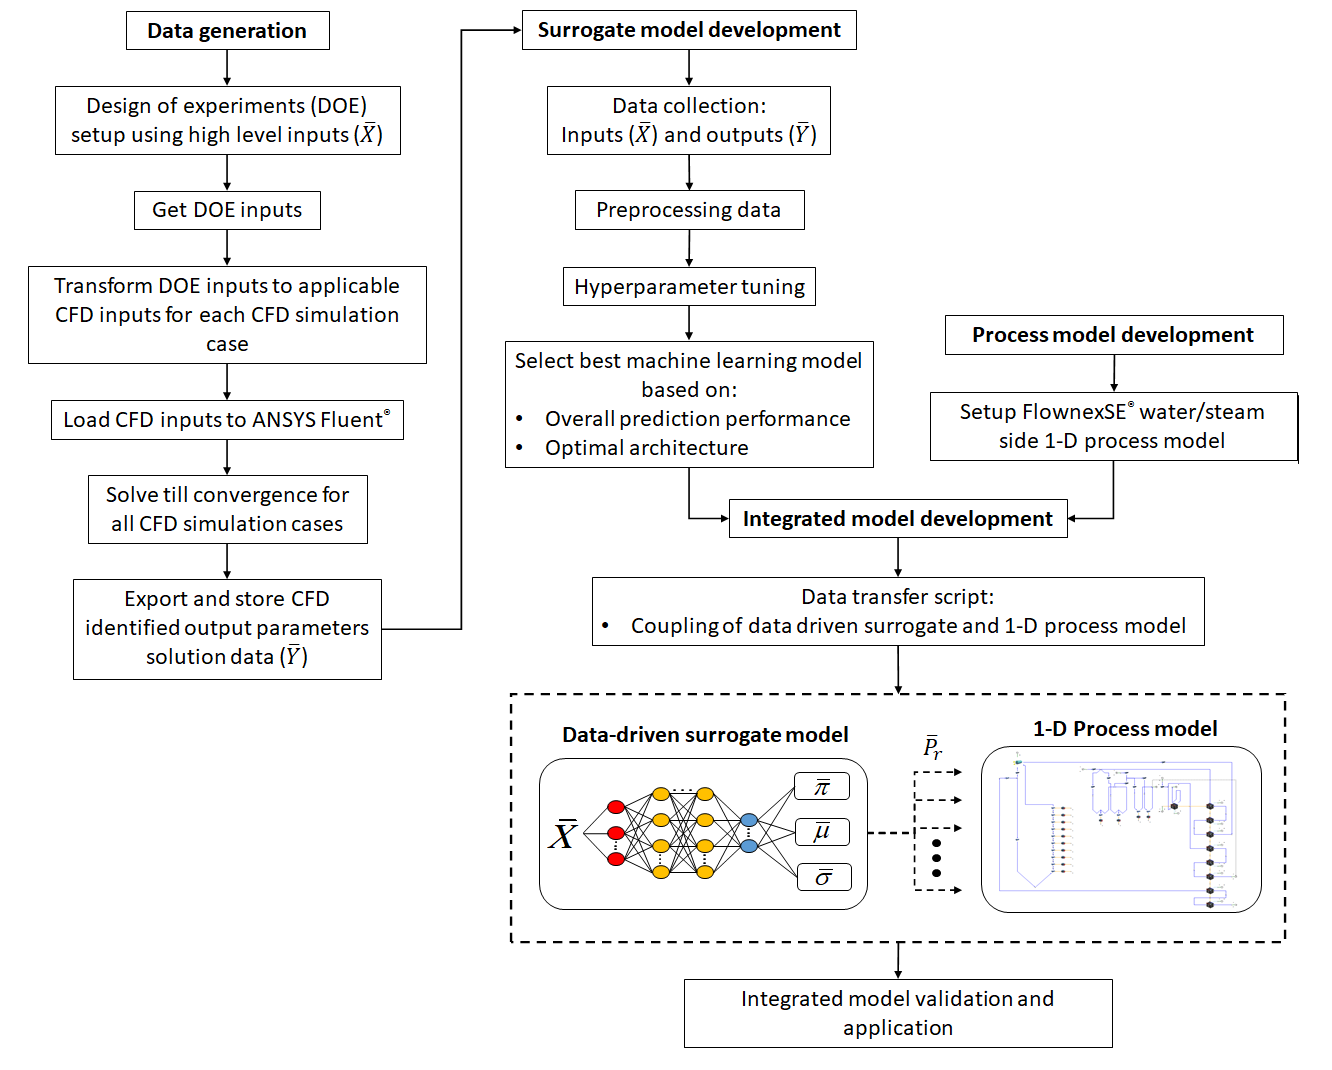
\includegraphics[scale=0.5]{WORK_FLOW}}
\caption{Summary of the model development process from data generation and collection to the final integrated model}
\label{fig_work_flow}
\end{figure}

Figure \ref{fig_work_flow} provides a flow chart that indicates the development process from the data generation and collection to the final integrated model development. The data generation process is further described in Section \ref{sec_data_gen}, which provides an evaluation of the 14 high level inputs ($\bar{X}$) and CFD output parameters ($\bar{Y}$) that are to be utilised in the surrogate model development. The surrogate model development is primarily covered by the machine learning theory discussed in Section \ref{sec_ml_theory} and the results of Section \ref{sec_hyper} which highlights the selection of the best machine learning model. Section \ref{sec_process} provides an overview of the developed 1-D process model. Thus, the remainder of this section will discuss the integrated models coupling and layout development.\\

In the current work a C\# script was used to access the Python application programming interface (API). This allows for the predictions ($\bar{P}_r$) to be made using the selected surrogate model developed in Python code. The predictions are retrieved using the script and transferred to the respective process model components as inputs. A schematic of the process model and its integration with the surrogate model is provided in Figure \ref{fig_int_model}. The process model accepts the predicted heat loads for the EV, SH2 and SH3 at interconnected boundary nodes, the same is illustrated for the flue gas state.\\
\begin{figure}[h!]
	\centering
		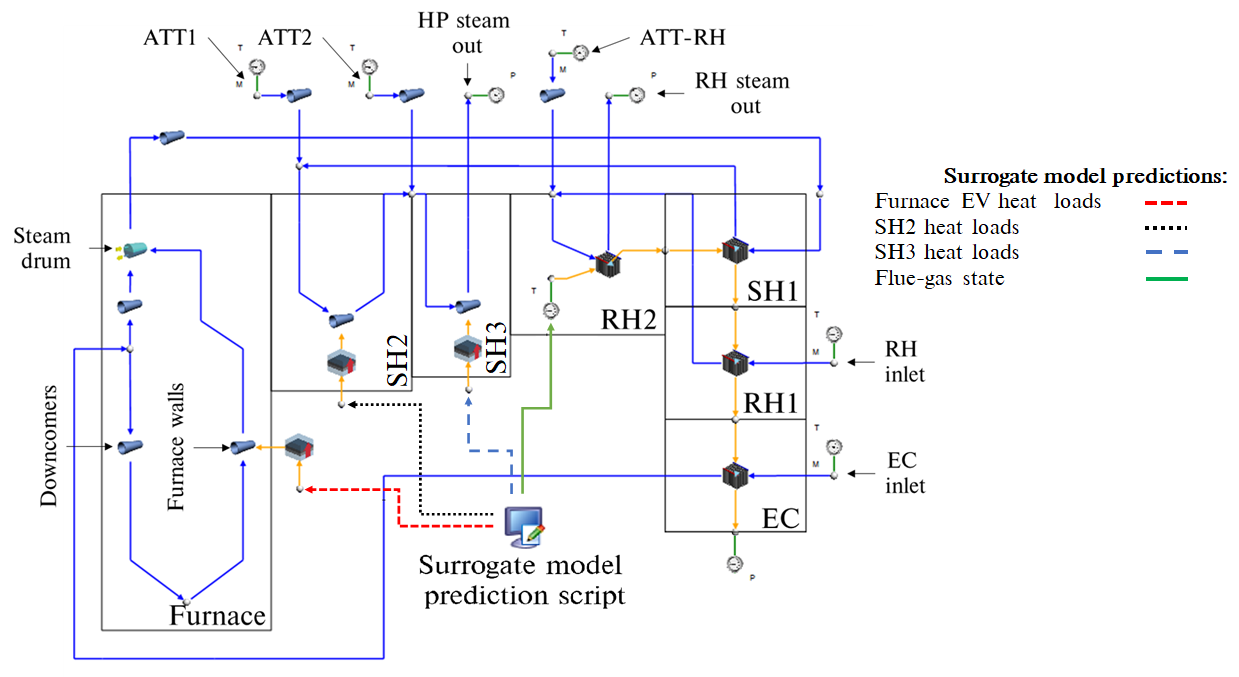
\includegraphics[scale=0.5]{INTEGRATED_MODEL}
	  \caption{Schematic of 1-D process model integrated with the data-driven surrogate model.}\label{fig_int_model}
\end{figure}

The boiler can be split into three sections namely, the furnace consisting of EV water walls, the radiative pass consisting of SH2 and SH3, and the convective pass consisting of RH2, SH1, RH1 and the EC. The furnace heat load predictions to the EV walls determine the evaporation rate. The high pressure (HP) steam outlet flow rate is calculated as the sum of the attemperation flow rates (ATT1 and ATT2) and the evaporation flow rate. The attemperators are used to control the steam temperature to ensure an exit temperature of 808 [$K$] at both the HP outlet and RH outlet. In addition to the furnace heat loads the surrogate model predicts the SH2 and SH3 heat loads. Lastly the surrogate model is able to predict the flue gas conditions at the inlet to the convective pass (i.e. RH2).
\newpage
\section{Applicable machine learning theory}\label{sec_ml_theory}
The present work makes use of various machine learning architectures to develop a surrogate model that can predict the thermal and combustion characteristics of a utility scale boiler using high level inputs. The current section discusses the details of the respective architectures, namely MLP and MDN machine learning models.
 
\subsection{Multilayer perceptron networks}
Artificial neural networks (ANN) are machine learning systems inspired by biological neural activity \cite{Rasmussen2006}. There are many classifications of ANNs, with multilayer perceptron networks (MLP) being the standard representation \cite{goodfellow}. Typically, MLPs are adapted for supervised learning problems where the input variables are mapped to labelled output variables. The relationship between the input and output variables are learned by optimizing the weights ($\overline{w}$) and biases ($\overline{b}$) to minimize a selected cost function, which for most cases is the MSE given in Equation \eqref{eqn_lin_cost}. A cost function usually calculates the difference between the estimated ($\hat{y_i}$) and the desired values and is reported as a single number \cite{Wheeler2019}.\\
\begin{equation}\label{eqn_lin_cost}
J_{MSE}=\frac{1}{n}\sum^n_{i=1}(y_i-\hat{y_i})^2
\end{equation} 

A standard MLP schematic is given in figure \ref{fig_mlp_schematic}, illustrating the common features of a MLP, that being the input, hidden and output layers.\\
\begin{figure}[h!]
	\centering
		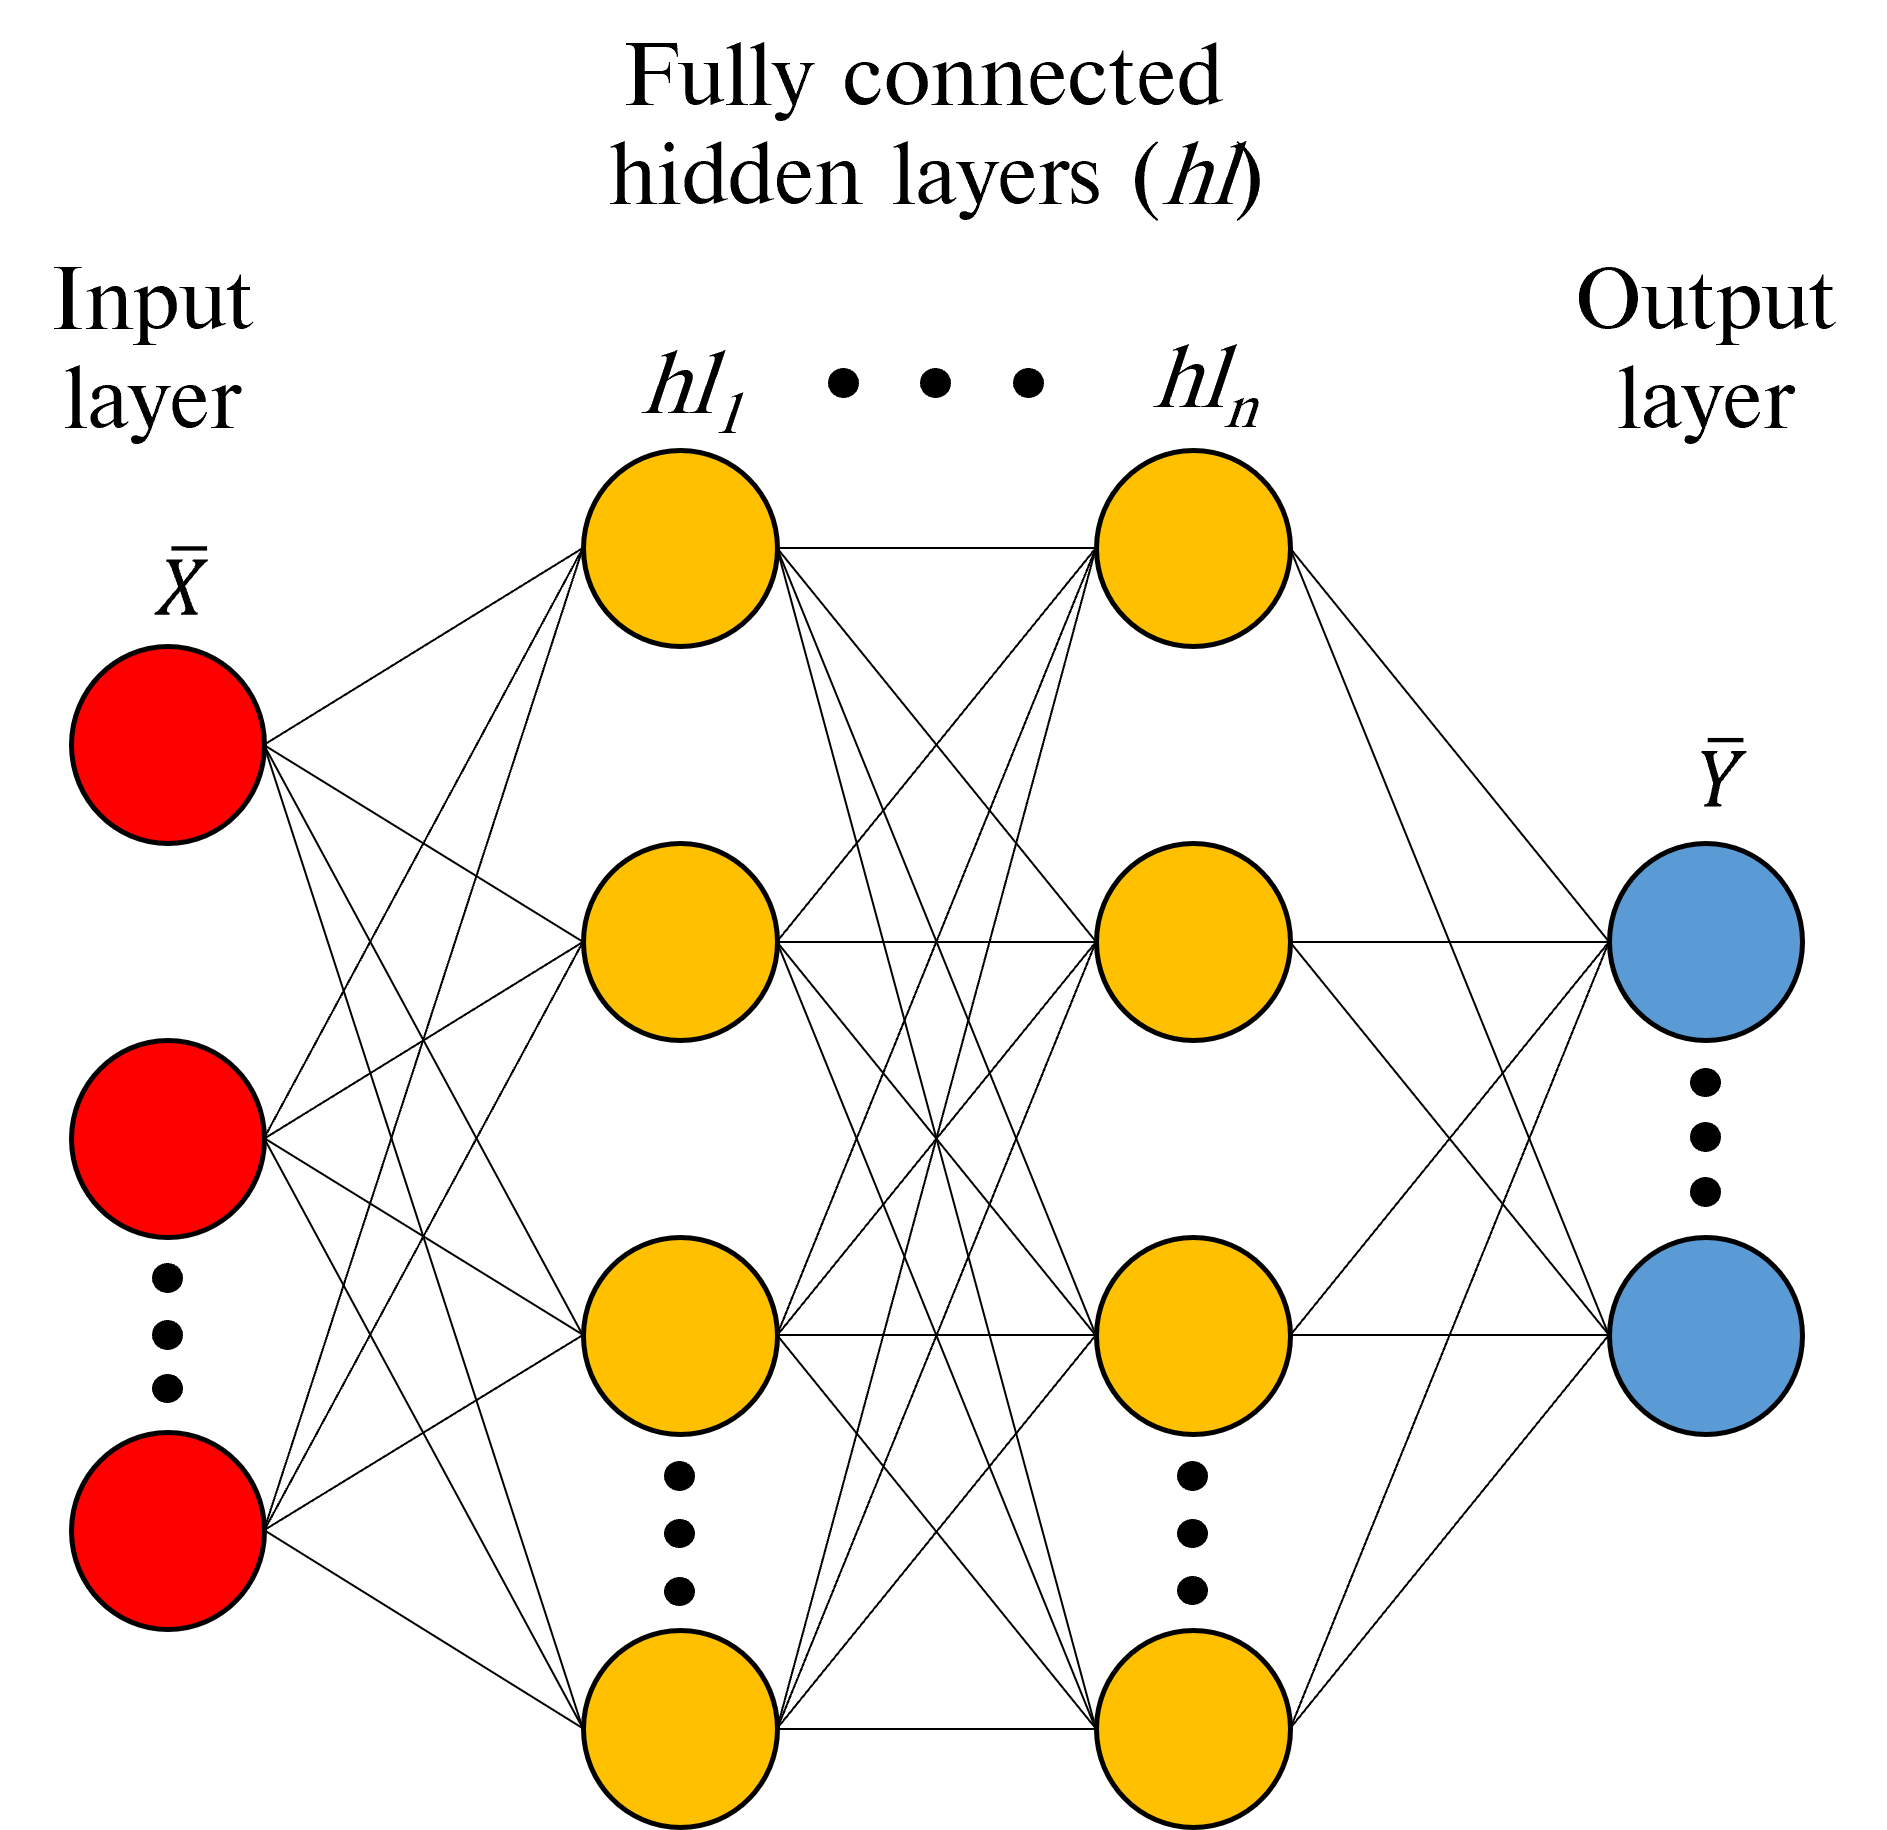
\includegraphics[scale=0.5]{ML_SCHEMATIC}
	  \caption{Traditional MLP schematic.}\label{fig_mlp_schematic}
\end{figure}

To calculate the output values ($\hat{y_i}$) the forward propagation algorithm is utilized, which calculates the output for each layer and moves sequentially through the network until an output is determined. Each network layer output is calculated using two steps, the first being the calculation of the summed signal ($\overline{z}_l$) and secondly the use of an activation function to generate the output signal ($\overline{h}_l$). Equation \eqref{eqn_summed_sig} highlights the first step, where $\overline{h}_{l-1}$ is the output signal from the previous layer.
\begin{equation}\label{eqn_summed_sig}
\overline{z}_l = \overline{h}_{l-1}\cdot\overline{w}_l+\overline{b}_l
\end{equation}

The result of equation \ref{eqn_summed_sig} is subsequently passed to an activation function ($\overline{h}_l = \sigma_l(\overline{z}_l)$). There are various activation functions that can be utilized, such as linear, ReLu, Elu, and the hyperbolic tangent \cite{goodfellow}, with the final layer activation function usually being linear for regression models. The current work makes use of ReLu for the hidden layers, since the ReLu are simple to implement and fast to compute \cite{Wheeler2019}, and a linear activation function for the output layer/s. The ReLu and linear activation functions are shown in Equation \ref{eqn_act_func}.
\begin{equation}\label{eqn_act_func}
\begin{split}
&\overline{h}_l=\sigma_{ReLu}(\overline{z}_l) = \overline{z}_l =  
	\begin{cases}
	 \overline{h}_{l-1}\cdot\overline{w}_l+\overline{b}_l\,\, &if\,\,\,\, \overline{z}_l>0\\
	 0\,\, &if\,\,\,\, \overline{z}_l<0
	\end{cases}\\
&\overline{h}_l=\sigma_{linear}(\overline{z}_l) = \overline{z}_l = \overline{h}_{l-1}\cdot\overline{w}_l+\overline{b}_l
\end{split}
\end{equation}

When the forward propagation step is complete, the network weights and biases can be updated to minimize the cost function (refer to Equation \eqref{eqn_lin_cost}) using the backward propagation method \cite{Rumelhart1986}. The methodology calculates the gradient of the cost function with respect to the weights and biases for each layer. Once the gradients have been calculated the weights and biases are updated using the gradient descent algorithm. The current work makes use of the Adam \cite{goodfellow} alternative to the gradient descent algorithm, which is illustrated in Equation \eqref{eqn_adam_algor}. Forward- and backward-propagation algorithms would be iteratively conducted until the cost function is reduced to below a desired threshold.
\begin{theorem} 
\begin{equation}\label{eqn_adam_algor} 
\begin{split}
&\overline{m}\leftarrow \beta_1\overline{m}+(1-\beta_1)\nabla_{\theta}J_{MSE}(\overline{\theta})\\
&\overline{s}\leftarrow \beta_1\overline{s}+(1-\beta_2)\nabla_{\theta}J_{MSE}(\overline{\theta})\otimes&\nabla_{\theta}J_{MSE}(\overline{\theta})\\
&\overline{m}\leftarrow\frac{\overline{m}}{1-\beta_1^t} \\
&\overline{s}\leftarrow\frac{\overline{s}}{1-\beta_2^t}\\
&\overline{\theta}\leftarrow\overline{\theta}-\eta\overline{m}\otimes(\sqrt{\overline{s}+\epsilon})^{-1}\\
\end{split}
\end{equation}
\end{theorem}

The variable $\bar{\theta}$ in Equation \eqref{eqn_adam_algor} represents the model weights and biases for each layer. Scaling ($\bar{s}$) and the momentum ($\bar{m}$) matrices are initialized to zero when beginning the training phase. The variable $t$ is the iteration counter, while $\beta_1$ and $\beta_2$ are the momentum and scaling decay hyper-parameters set to values of 0.9 and 0.999 respectively. Lastly $\epsilon$ is a smoothing term set to a value of $10^{-8}$. In the present work various learning rates ($\eta$) were investigated during the hyper-parameter search for both the MLP and MDN neural architectures.

\subsection{Mixture density networks (MDNs)}
Mixture density networks are fundamentally built from two components, namely an ANN and a mixture model. This allows for multi-modal predictions. The ANN can be a standard feed-forward MLP or a recurrent neural network (RNN), with RNNs being used in transient applications with at least one feedback loop \citep{Oko2015}.\\

MDNs are used to predict the parameters of a probability distribution ($P(\overline{X}\mid\overline{Y})$), allowing for non-Gaussian distributions to be modelled, thus making MDNs a probabilistic machine learning framework. MDNs estimate the conditional probability distribution as a mixture of Gaussian distributions where the mixing coefficients ($\overline{\pi}_k$) and component densities are flexible functions of the input data ($\overline{X}$). Equation \eqref{eqn_cond_prob_func} illustrates the conditional probability function.
\begin{equation}\label{eqn_cond_prob_func}
P(\overline{X}\mid\overline{Y}) = \sum_{k=1}^K\overline{\pi}_k(\overline{X})\cdot \mathbb{N}(\overline{Y}\mid \overline{\mu}_k(\overline{X}),\overline{\sigma}_k(\overline{X}))
\end{equation}
where $K$ represents the number of selected normal distributions, while $\overline{\mu}_k$ and $\overline{\sigma}_k$ are the predicted means and standard deviations for each distribution $k$ given the input data $\overline{X}$ respectively.\\

A schematic of a simple MDN network is given in Figure \ref{fig_mdn_schematic}, highlighting the mixing coefficients, predicted means and deviations. It is shown that modifications are made to the output layer by splitting the network output into three parts to calculate the $\overline{\pi}_k$, $\overline{\mu}_k$ and $\overline{\sigma}_k$ for each $k$ distribution. This enables the MDN network to learn the $P(\overline{X}\mid\overline{Y})$.\\
\begin{figure}[h!]
	\centering
		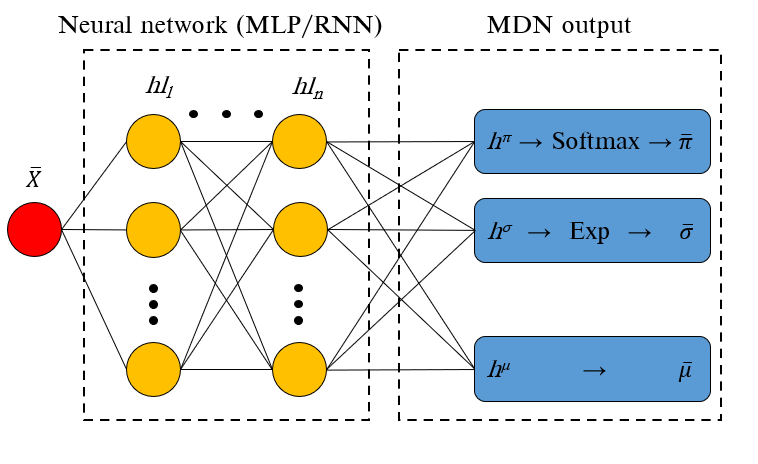
\includegraphics[scale=0.5]{MDN_SCHEMATIC}
	  \caption{Simple MDN network.}\label{fig_mdn_schematic}
\end{figure}

Bishop \cite{bishop1994} proposed the following restrictions for the mixing coefficients and variance components of the MDN output layer. Since the mixing coefficients contain the discrete probabilities of an output belonging to each $K$ normal distribution for all observations, the mixing coefficients must satisfy the constraints listed in Equation \eqref{eqn_mix_coef_constraint}.
\begin{equation}\label{eqn_mix_coef_constraint}
\begin{split}
&\sum_{k=1}^K\overline{\pi}_k^n=1\\
&0\leq\overline{\pi}_k^n\leq1
\end{split}
\end{equation}
These constraints are met by using a \textit{softmax} function on the output of the hidden layer $h^{\pi}$. The mixing coefficient is calculated using Equation \eqref{eqn_mix_coeff}.
\begin{equation}\label{eqn_mix_coeff}
\overline{\pi}_k^n(\overline{x}^n)=\frac{exp(h_k^{\pi,n})}{\sum_{k=1}^Kexp(h_k^{\pi,n})}
\end{equation}

Similarly, a constraint is applied to the standard deviation values ensuring a positive value, this is achieved using an exponential function being applied to the standard deviation leg of the MDN output layer, namely $h^{\sigma}$. Equations \eqref{eqn_stddev} shows the imposed constraint for the standard deviation leg.\\
\begin{equation}\label{eqn_stddev}
\begin{split}
&(\overline{\sigma}^n_k(\overline{x}^n))^2\geq 0\\
&\sigma_k^n(\overline{x}^n)=exp(h_k^{\sigma,n})
\end{split}
\end{equation}

The MDN weights and biases are optimized by minimizing the negative log-likelihood for all observations in a batch. This is shown in Equation \eqref{eqn_nll}.
\begin{equation}\label{eqn_nll}
J_{NLL}(\overline{Y},\overline{\pi},\overline{\sigma},\overline{\mu})=-\sum^N_{n=1}ln\left\{\sum^K_{k=1}\overline{\pi}_k(\overline{X}^n,\overline{\theta})\cdot \mathbb{N}(\overline{Y}^n\mid\overline{\mu}_k(\bar{X}^n,\bar{\theta}),\overline{\sigma}^2_k(\overline{X}^n,\overline{\theta})) \right\}
\end{equation}
\section{Data generation}\label{sec_data_gen}
The steady-state multiphase non-thermal equilibrium CFD model, discussed in Section \ref{sec_cfd} was used to generate the training and testing data, which was subsequently used for training/testing of an appropriate data-driven surrogate model.

\subsection{Simulated dataset}
The high-level inputs to the surrogate model include the following: the excess air ratio, the fuel flow rate for the six mills in operation, the average steam temperatures for SH2 and SH3, the fouling resistance for SH2 and SH3, the proximate composition of ash and moisture of the fuel and the higher heating value (HHV) of the fuel, which is a function of the fuel composition determined using the Dulong equation \cite{Ganapathy2014}. Thus, the input field has a dimensionality of $d_{inputs}=14$. To obtain a representative set of results for training and testing the surrogate model, a design of experiments (DOE) was conducted to generate a set of 180 unique simulation cases. The various high-level input ranges used in the DOE are provided in Table \ref{tbl_doe}. The ranges where selected to cover a wide range of operational loads with maximum continuous ratings (MCR) between 100\% and 30\%. The DOE matrix was populated using the latin hypercube sampling method provided in the Python \textit{pyDOE} 0.3.8 library.
\begin{table}[pos =h]
\caption{Design of experiments input ranges for CFD simulations}\label{tbl_doe}
\begin{tabular*}{0.8\textwidth}{p{0.3\textwidth}p{0.1\textwidth}p{0.1\textwidth}p{0.1\textwidth}l}
\hline
\toprule
 Input variables& Mean & Min& Max& Units \\ % Table header row
\midrule
Total fuel flow rate*, ($\sum_{i=1}^6\dot{m}_{fuel,i}$)&68.9 & 39.5 & 120.2 & $kg/s$ \\
Fuel moisture content, ($Y_{H_2O}$) &0.056& 0.025 & 0.085 & $kg/kg$ \\
Fuel ash content, ($Y_{ash}$)  &0.418& 0.259 & 0.559 & $kg/kg$ \\
SH2 fouling resistance, ($R_{SH2}$)  &0.006& 0.004 & 0.007 & $K/W$ \\
SH3 fouling resistance, ($R_{SH3}$)  &0.014 &0.008 & 0.017 & $K/W$ \\
Higher heating value, ($HHV$)&14.987&12.535 & 19.105&$MJ/kg$\\
Excess air, ($\gamma_{air}$) &1.145& 1.101 & 1.272 & $\%$\\
SH2 steam temperature, ($\overline{T}_{SH2}$)&701& 686 & 717 & $K$\\
SH3 steam temperature, ($\overline{T}_{SH3}$)&781 &768 & 796& $K$\\
\bottomrule
*\small{Sum of the 6 mill fuel flow rates}
\end{tabular*}
\end{table}

The resultant matrix of 180 simulation cases would then be transformed into appropriate CFD inputs, as indicated in Figure \ref{fig_work_flow}. These 180 unique CFD cases were subsequently run using 216 Intel\textsuperscript{\textregistered} Xeon\textsuperscript{\textregistered} 2.6 GHz cores, made available by the Centre for High-Performance Computing, South Africa. Once the CFD simulations achieved convergence, the target data, comprising of the discretised heat loads to the furnace, platen SH and final SH, the exit flue gas temperatures and flue gas composition, was stored for each case. A schematic of the output data reporting surfaces is given in Figure \ref{fig_cfd_output}, and highlights the 10 discretised EV wall sections, the two tube bank legs making up both SH2 and SH3 superheaters, as well as the SH3 exit plane where the mass weighted flue gas state variables are reported.\\

A total of 22 output target values ($d_{targets}$) are extracted from the results for each CFD simulation case. Due to the inherently unsteady nature of the CFD simulations monitored values, even when convergence has been achieved, the output target values were extracted after every 50 iterations for an additional 2500 iterations once convergence was achieved. This results in each CFD simulation case having a solution data matrix size of ($\bar{Y}\in \mathbb{R}({50\times d_{targets}})$). Table \ref{tbl_output_cfd} provides a statistical summary of the target data that was generated from the 180 CFD simulations, subsequently the data was pre-processed and cleaned to eliminate any unrealistic operational conditions.
\newpage
\begin{figure}[h!]
\centerline{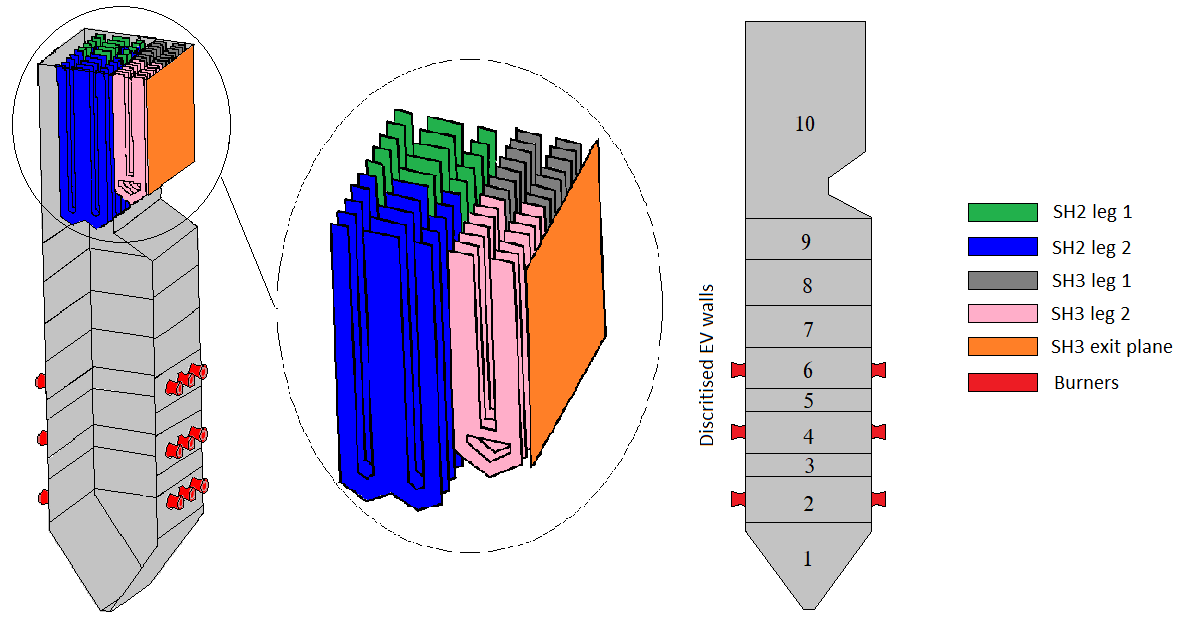
\includegraphics[scale=0.4]{DIST_WALL}}
\caption{CFD solution data reporting surfaces, including the ten discretised EV wall sections, the SH2 and SH3 tube bank split and the SH3 exit plane.}\label{fig_cfd_output}
\end{figure}
\begin{table}[pos = h]
\centering
\caption{Summary of the CFD generated output data}
\label{tbl_output_cfd}
\begin{tabular*}{\textwidth}{p{0.25\textwidth}p{0.13\textwidth}p{0.13\textwidth}p{0.13\textwidth}p{0.13\textwidth}p{0.09\textwidth}}
\toprule
\textbf{Output variables} & \textbf{Mean}&\textbf{Std. deviation} & \textbf{Min} & \textbf{Max} & \textbf{Units} \\
\hline
\multicolumn{6}{c}{\textit{Heat loads}}\\
\hline
Wall - 1 &$30.76$ &$25.85$& $1.01$ & $98.12$ & $MW$\\
Wall - 2 &$21.56$ &$7.68$& $0.84$ & $43.24$ & $MW$\\
Wall - 3 &$20.85$ &$8.03$& $1.17$& $38.37$& $MW$\\
Wall - 4 &$29.17$ &$8.82$& $5.20$& $46.99$& $MW$\\
Wall - 5 &$22.77$ &$8.61$& $4.70$& $43.24$& $MW$\\
Wall - 6 &$30.97$ &$10.19$& $4.95$& $52.99$& $MW$\\
Wall - 7 &$39.92$ &$14.26$& $10.98$& $84.82$& $MW$\\
Wall - 8 &$38.70$ &$11.06$& $13.66$& $67.89$& $MW$\\
Wall - 9 &$30.62$ &$8.22$& $11.78$& $52.06$& $MW$\\
Wall - 10 & $78.06$ &$20.70$& $30.04$ & $148.02$& $MW$\\
SH2 leg - 1 &$65.96$ &$25.47$& $13.70$&$124.01$ & $MW$\\
SH2 leg - 2 &$78.98$ &$26.13$&$15.56$ & $132.30$& $MW$\\
SH3 leg - 1 &$23.65$ &$7.97$&$2.63$ &$45.12$ & $MW$\\
SH3 leg - 2 & $24.46$&$7.58$&$3.80$ &$43.75$ & $MW$\\
Roof &$12.14$ &$3.34$&$3.15$ &$22.81$ & $MW$\\
\hline
\multicolumn{6}{c}{\textit{Flue gas composition and exit state}}\\
\hline
$Y_{CO_2}$& 0.188&0.025&0.126 & 0.235& $kg/kg$\\
$Y_{H_2O}$& 0.041&0.005& 0.031&0.051 & $kg/kg$\\
$Y_{O_2}$&0.062 &0.020&0.023 &0.117 & $kg/kg$\\
$Y_{SO_2}$&$2.47\times10^{-3}$ &$3.2\times10^{-3}$& $1.73\times10^{-3}$& $3.02\times10^{-3}$& $kg/kg$\\
Temperature, ($T_{fg,exit}$) &1143 &109&894 &1417 & $K$\\
Mass flow rate, ($\dot{m}_{fg,exit}$) & 514.6 &102.9& 298.3& 791.8 & $kg/s$\\
Incident radiation, ($G_{exit}$)& $399.0$ &$126.5$& $126.7$ & $750.8$ & $kW/m^2$\\
\hline
\end{tabular*}
\end{table}
\newpage
\section{Results and discussion}\label{sec_results_diss}
The following section provides the results of the hyperparameter tuning conducted in the development of the of the data-driven surrogate model using the generated CFD solution dataset of Section \ref{sec_data_gen}. Utilising the best machine learning model, the integrated model, as discussed in Section \ref{sec_int_model}, was developed via the coupling of the 1-D process model of the water-/steam-side and the developed data-driven surrogate model. In addition, the results of a validation case study using experimental data was conducted for a wide range of loads. Finally, the results of an application case study, utilising the integrated model, was conducted that investigates the effects of fuel quality have on the integrated boiler performance.
\subsection{Hyper-parameter tuning \& final model selection}\label{sec_hyper}
The present work makes use of two types of machine learning models, namely a standard MLP and a mixture density designated model connected to a standard MLP (MDN). The following section will discuss the hyper parameter tuning and final selected model configuration. The programming language Python 3.7.8 and the \textit{Tensorflow} 2.6.1 machine learning libraries were utilised in the present study.\\

The total CFD solution data matrix size will consist of $180\times\overline{Y}=198000$ data points. Using the total solution data matrix for training and testing would typically result in a slower convergence \cite{goodfellow}. However, the use of subset data packages, referred to as batches or mini-batches, allows for a faster convergence. The batch size is a term used in machine learning that specifies a number of training/testing examples utilized in one iteration \cite{Wheeler2019}. Thus, for a data batch size, $m_b$, the output tensor for the MLP model will be $\hat{Y}\in \mathbb{R}({m_b\times d_{targets}}$). However, the output data for the MDN model will consist of three parts, namely; the mixing coefficients tensor of shape  $\bar{\pi}\in \mathbb{R}({m_b \times K})$, the output standard deviation tensor of shape $\bar{\sigma}\in \mathbb{R}({K\times m_b\times d_{targets}})$, and the predicted means of tensor shape $\bar{\mu}\in \mathbb{R}({K\times m_b\times d_{targets}})$, where $K$ is the number of distributions. The input data fed into both the MLP and MDN will have shape $\bar{X}\in \mathbb{R}({m_b\times d_{inputs}})$. The target dataset was split with 80\% of the data being used for training purposes and the remainder for testing. To reduce the training time of the neural networks a min-max normalization was utilized to scale all the dataset entries to values between $0\rightarrow1$.\\

Table \ref{tbl_tuning} highlights the hyper-parameter search spaces for both the MLP and MDN model. The MDN has an added parameter, namely the number of additional distributions that the MDN would need to fit to the output data. The hyper-parameter tuning of both the MLP and MDN models made use of 1000 epochs. This was deemed adequate to train/test the models for the various hyper-parameter search spaces and was utilized to reduce the computational effort/time.
\begin{table}[pos=h]
\caption{Hyper-parameter search space for fully connected MLP and MDN models}\label{tbl_tuning}
\begin{tabular*}{0.8\textwidth}{p{0.3\textwidth}p{0.24\textwidth}p{0.24\textwidth}}
\toprule
 Parameter& MLP search space & MDN search space \\ % Table header row
\midrule
 Number of distributions & - & 1,2,3,4  \\
 Number of layers & 2,3,4 & 2,3,4\\
 Number of neurons per layer & 10, 40, 80, 100  & 10, 40, 80, 100\\
 Learning rates & 1e-3, 1e-4, 1e-5, 1e-6 &  1e-3, 1e-4, 1e-5, 1e-6   \\
 Mini batch sizes  &32, 64, 128, 256 &32, 64, 128, 256  \\
\bottomrule
\end{tabular*}
\end{table}

The hyper-parameter search was conducted in a sequential manner with the MAEs, and root mean square errors (RMSE) being taken as important performance indicators for each trained case. Firstly, the hidden layer architecture of both models (MLP \& MDN) was varied by considering the number of hidden layers and neurons per layer. Figure \ref{fig_mlp_hyper} (a) illustrates the MLP model performance for the various hidden layer architectures. The neuron capacity reaches a minimum MAE at 80 neurons per layer for a 4-layer architecture. Further increasing the neuron capacity results in an increase in the MAE, possibly indicating an over fitting of data. Secondly, the learning rates were varied for the best performing architecture of the first hyper-parameter tuning step.\\
\newpage
Considering Figure \ref{fig_mlp_hyper} (b), a decrease in the learning rate shows an improvement in the MAE, with a learning rate of $1\times10^{-5}$ being the best for the current epoch size. For comparative purposes, learning rates of $1\times10^{-5}$ and $1\times10^{-6}$ were used in the final step, where the mini-batch sizes are varied. Figure \ref{fig_mlp_hyper} (c) highlights the comparison for a fixed epoch, with a mini-batch size of 32 and a corresponding learning rate of $1\times10^{-5}$ showing the best MAE improvement.
\begin{figure}[h!]
\centering
    \begin{subfigure}{0.48\textwidth}
    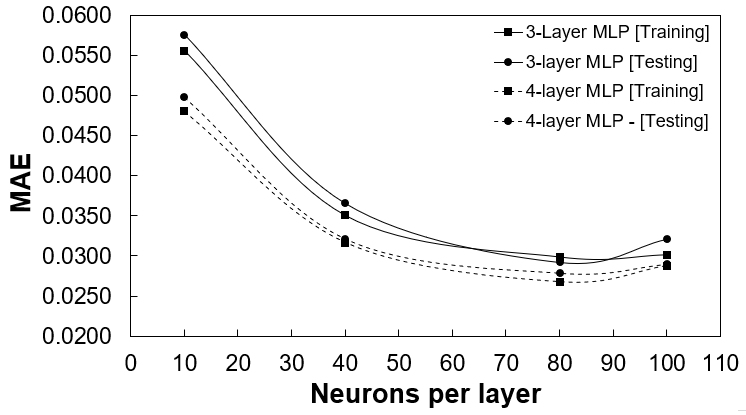
\includegraphics[width=1\textwidth]{NEURONS_HYPER}
    \caption{}
    \end{subfigure}
        \begin{subfigure}{0.48\textwidth}
    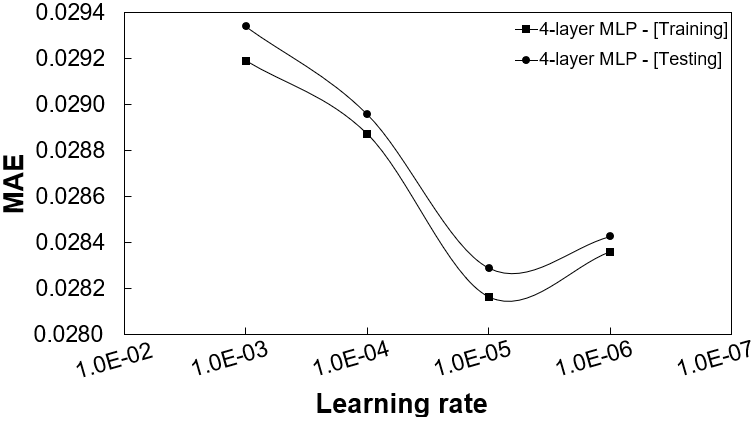
\includegraphics[width=1\textwidth]{LR_HYPER}
    \caption{}
    \end{subfigure}\\
        \begin{subfigure}{0.48\textwidth}
    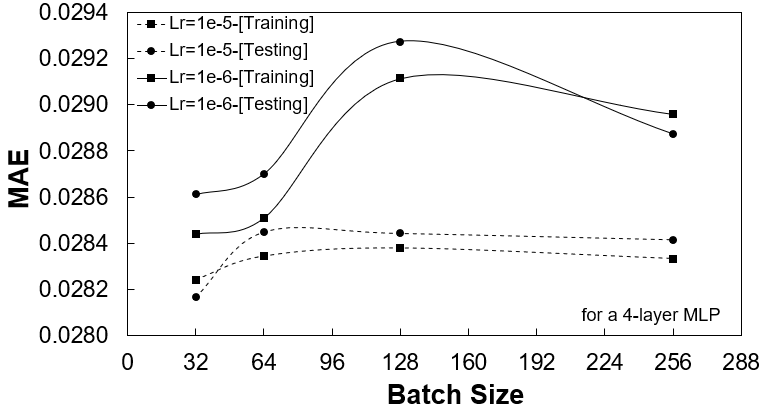
\includegraphics[width=1\textwidth]{BATCH_SIZE_HYPER}
    \caption{}
    \end{subfigure}
    \caption{MLP model performance for; (a) hidden layer architecture, (b) varying learning rates, and (c) varying mini-batch sizes.}\label{fig_mlp_hyper}
\end{figure}

The MDN hyper-parameter tuning was conducted in a similar manner except that an additional step was required. This was to consider the number of distributions the MDN would use to capture the probabilistic characteristics. Figure \ref{fig_mdn_hyper} shows the MAE for the various distributions, with a distribution of one representing the best MLP model. An increase in the number of distributions tends to improve the MAE, however it is evident that a threshold of 3 distributions results in the best improvement.\\
\begin{figure}[h!]
	\centering
		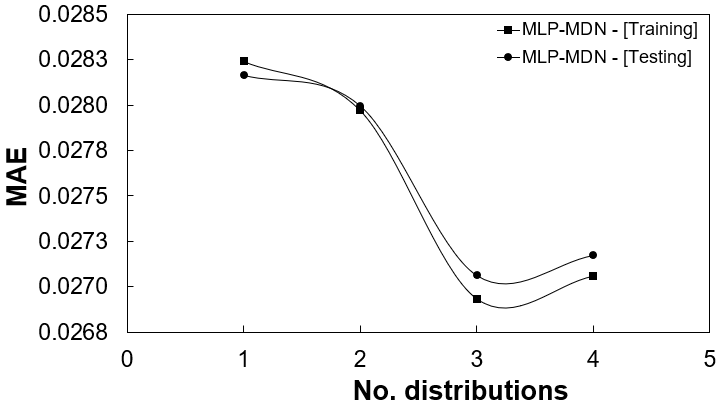
\includegraphics[width=0.48\textwidth]{DIST_HYPER}
	  \caption{MDN model performance for number of distributions.}\label{fig_mdn_hyper}
\end{figure}

\begin{table}[h!]
\centering
\caption{Hyper-parameter search results}\label{tbl_hyper_results}
\begin{tabular*}{0.6\textwidth}{p{0.3\textwidth}p{0.15\textwidth}p{0.15\textwidth}}
\toprule
 Parameter& MLP & MDN \\ % Table header row
\midrule
 Number of distributions & - & 3  \\
 Number of layers & 4 & 4\\
 Number of neurons per layer & 80  & 80\\
 Learning rate & 1e-5 &  1e-5   \\
 Mini batch size  &32 & 32  \\
\midrule
Errors & &\\
\midrule
RMSE & 0.0213 & 0.0211\\
MAE & 0.0282& 0.0263\\
\bottomrule
\end{tabular*}
\end{table} 

The results of hyper-parameter search are given in Table \ref{tbl_hyper_results}. Unlike the MLP, which can only produce a single set of predictions for an input, the MDN is able to produce a distribution of predictions based on the most probable mixing coefficient. This highlights one of the main advantages of the using the MDN model, which is its ability to learn the uncertainty that comes from using a probabilistic model that enables the modelling approach to take into account the effect information density in the training data. This is shown in the error distributions graphs of Figures \ref{fig_frequency_data} (a) and (b). For the MDN model it is seen that approximately 80-90\% of the training data has mean absolute percentage errors (MAPEs) below 10\%, with the MLP model showing a similar trend.\\
\begin{figure}[h!]
\centering
    \begin{subfigure}{0.48\textwidth}
    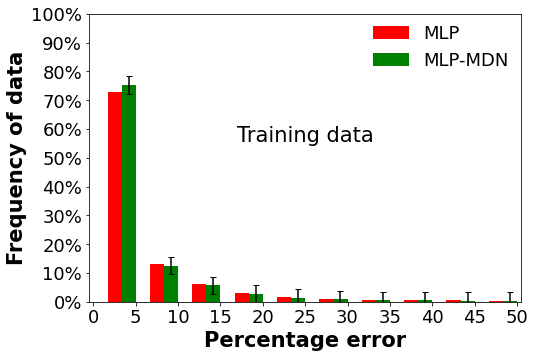
\includegraphics[width=\textwidth]{OVERALL_TRAIN}
    \caption{}
    \end{subfigure}
    \begin{subfigure}{0.48\textwidth}
    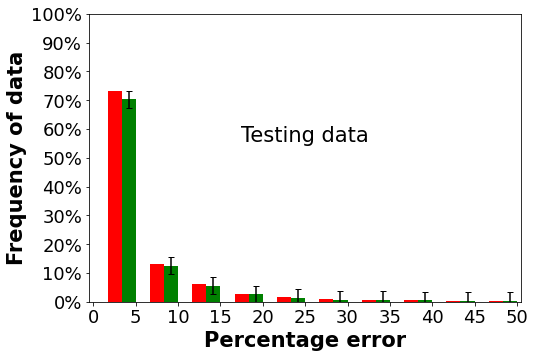
\includegraphics[width=\textwidth]{OVERALL_TEST}
    \caption{}
    \end{subfigure}
    \caption{Overall error distributions for the selected MLP and MDN model; (a) training data and (b) testing data.}\label{fig_frequency_data}
\end{figure}

Based on the above analysis, the MDN model was selected as the best model to be used for the surrogate model implementation. The benefit of using the MDN surrogate model is the ability to provide not only the expected mean (most-probable) value of each output parameter, but also the associated standard deviation. Having the mean value of each of the furnace and heat exchanger heat loads together with its uncertainty in the form of a standard deviation, allows the uncertainty to be propagated through the entire integrated model. It is therefore possible to obtain the resultant mean values of the overall plant performance parameters together with their uncertainties emanating from the surrogate model prediction.
\newpage
\subsection{Validation of integrated model using experimental data}\label{sec_result_1}
The results predicted using the surrogate model were validated for the 100\%, 80\% and 60\% MCR load cases. Measured data were made available for these load cases, which allow the mean and standard deviation to be determined.  The mean and standard deviation of each output can then be compared with the predicted mean and standard deviation obtained with the integrated model.\\

The most probable predictions of the surrogate model can only be used to estimate the mean and standard deviation values for the EV, SH2 and SH3 wall heat loads. However, to propagate the uncertainty of the most probable predictions and ascertain the summary statistics for the convective section heat exchangers (RH2, SH1, RH1 and EC), as well as the steam generation rates and the attemperator flow rates, the Monte Carlo method was utilised. The Monte Carlo method is a mathematical technique used to estimate the outcome of a given stochastic process \cite{Cheen2017}. In the current work the integrated model was applied in conjunction with the Monte Carlo method \cite{Thomopoulos2013}. Firstly, random sampling of the input variables to the integrated model are performed based on the mean and standard deviation predicted by the surrogate model.  Following this, simulations are run for each sample and the outputs are evaluated to determine the predicted mean and standard deviation of each overall plant parameter.\\

Fortunately, FlownexSE\textsuperscript{\textregistered} 2021, provides a built-in Monte Carlo facility. It requires as input the mean and standard deviation values for each model input \cite{flownex}. The Monte Carlo model inputs used in this study are the predicted mean and standard deviation results obtained with the data-driven surrogate model. Table \ref{tbl_inputs} illustrates the high-level MDN input vectors ($\overline{X}$) utilised for the validation and off-design case studies. For this study $N=1000$ Monte Carlo simulations were performed for each validation load.\\
\begin{table}[pos = h]
\caption{MDN input vectors ($\overline{X}$) for the validation and the off-design fuel case studies}\label{tbl_inputs}
\begin{tabular*}{0.9\textwidth}{p{0.14\textwidth}p{0.1\textwidth}p{0.1\textwidth}p{0.1\textwidth}p{0.1\textwidth}p{0.1\textwidth}p{0.15\textwidth}}
\hline
\multicolumn{2}{l}{}& \multicolumn{3}{c}{\textbf{Validation load cases}}&\multicolumn{2}{c}{\textbf{Varied fuel load cases}}\\
\multicolumn{2}{l}{\textit{Input variables}} & 100\%  & 81\% & 60\% & High-ash & High-moisture  \\
\hline
\multicolumn{2}{l}{Excess air content} & 1.155 & 1.209 & 1.263 & 1.155 & 1.155  \\
\multicolumn{2}{l}{$Y_{ASH}$ - [$kg/kg$]} & 0.409 & 0.409 &  0.409 &0.501 & 0.409 \\
\multicolumn{2}{l}{$Y_{H_{2}O}$ - [$kg/kg$]} & 0.055 & 0.055 & 0.055 & 0.055 & 0.150  \\
\multicolumn{2}{l}{HHV - [$MJ/kg$]} & 15.07 & 15.07 & 15.07 & 13.21 & 13.09  \\
\multicolumn{2}{l}{$R_{SH2}$ - [$K/W$]}& 0.012 & 0.012 & 0.012 & 0.012 & 0.012  \\
\multicolumn{2}{l}{$R_{SH3}$ - [$K/W$]} & 0.0067&0.0067 &0.0067 & 0.0067&0.0067  \\
\multicolumn{2}{l}{SH2 steam temperature - [$K$]} & 698 &697&781 &698 &698  \\
\multicolumn{2}{l}{SH3 steam temperature - [$K$]}& 787 & 793 &781 &787 &787  \\
\hline
\multicolumn{7}{c}{\textit{Mill flow rates} - [$kg/s$]}\\
\textbf{MCR load}& \textbf{Mill 1}& \textbf{Mill 2}& \textbf{Mill 3}& \textbf{Mill 4}& \textbf{Mill 5}& \textbf{Mill 6}\\
\hline
100\%& 19.14& 20.22& 19.92& 19.98& 19.41& 0.00\\
81\%& 18.23& 19.72& 19.02& 17.82& 18.02& 0.00\\
60\%& 15.46& 16.13& 0.00& 15.11& 15.32& 0.00\\
\hline
\end{tabular*}
\end{table}  

Figures \ref{fig_heat_load} - \ref{fig_attemp} provide comparative results of the measured data and integrated model responses for all three MCR load cases. Included on all the plots are confidence bands which represent the range/spread of data for each variable. Figures \ref{fig_heat_load}(a) to (c) show the integrated model's response for the total heat loads to the various heat exchangers for the 100\%, 80\% and 60\% MCR loads.\\
\begin{figure}[h!]
\centering
\begin{subfigure}{0.33\textwidth}
    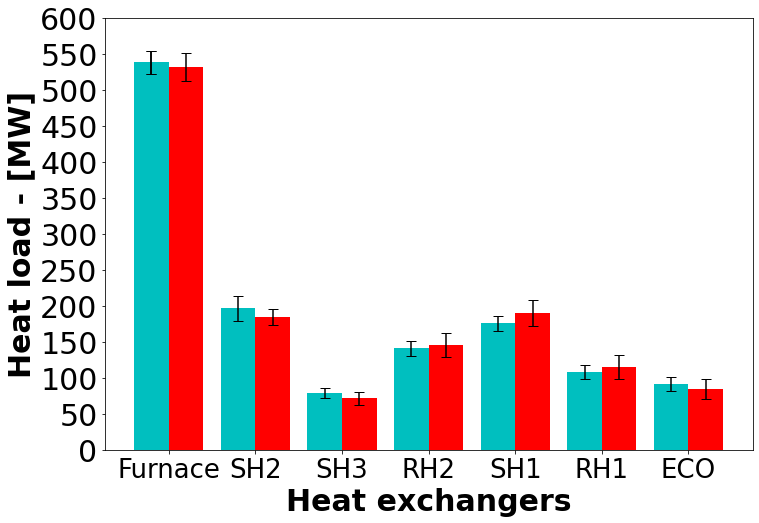
\includegraphics[width=\textwidth, height = 4.25cm]{100_CASE}
    \caption{100\% MCR}
\end{subfigure}\hfill % maximize horizontal separation
\begin{subfigure}{0.33\textwidth}
    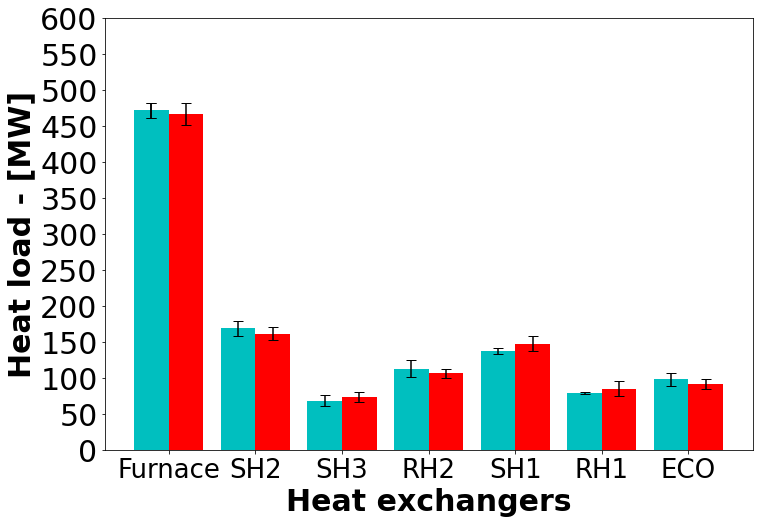
\includegraphics[width=\linewidth, height = 4.25cm]{80_CASE}
    \caption{80\% MCR}
\end{subfigure}\hfill
\begin{subfigure}{0.33\textwidth}
	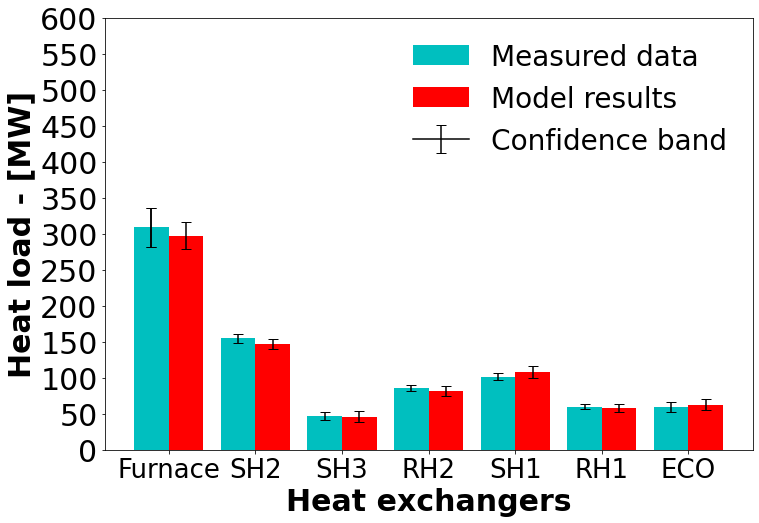
\includegraphics[width=\linewidth, height = 4.25cm]{60_CASE}
        \caption{60\% MCR}
\end{subfigure}
\caption{Load validation result comparison of the measured data and MDN model results for the various heat exchangers}
\label{fig_heat_load}
\end{figure}
\newpage
For the 100\% MCR load, the integrated model under predicts the mean results of
the heat loads in the radiative section (EV, SH2 and SH3) by a maximum of 4\%, which is realised in SH2 (approximately 8 [$MW$] for a mean SH2 heat load of 196 [$MW$]). Furthermore, the model over predicts the mean heat loads to the convective section (RH2 through EC) with a maximum deviation of 7\%, which is realised in SH1 (approximately 10 [$MW$] for a mean SH1 heat load of 175 [$MW$]). A similar trend is realised for 80\% and 60\% MCR loads, with the former showing an over prediction of 4\% of the mean heat load to SH3. However, the associated uncertainty of the integrated model overlaps with the measured data uncertainty with minimal outliers, therefore, inferring that the model
predictions are sufficiently accurate, this is illustrated by comparing the confidence band intervals of the measured and model results.\\
\begin{figure}[h!]
\centering
\begin{subfigure}{0.33\textwidth}
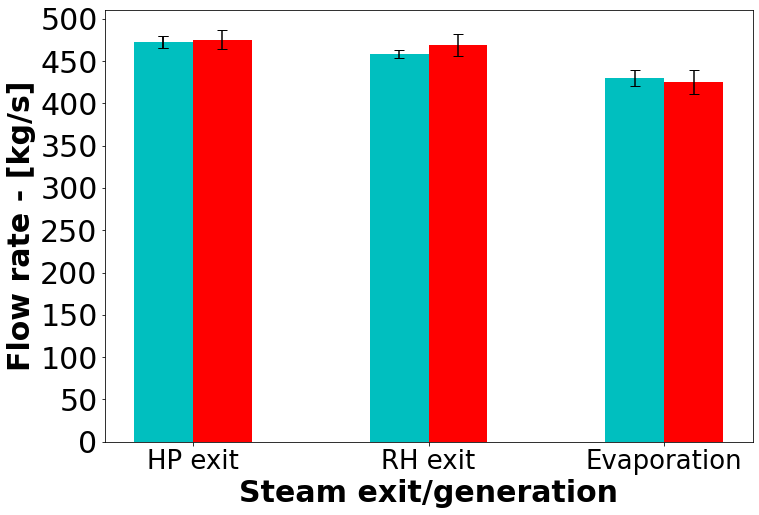
\includegraphics[width=\linewidth, height = 4.25cm]{100_CASE_STEAM}
        \caption{100\% MCR}
\end{subfigure}\hfill % maximize horizontal separation
\begin{subfigure}{0.33\textwidth}
    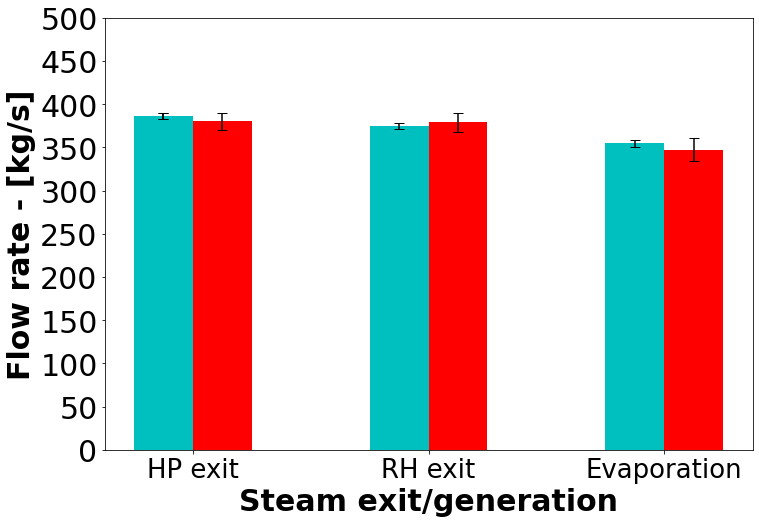
\includegraphics[width=\linewidth, height = 4.25cm]{80_CASE_STEAM}
    \caption{80\% MCR}
\end{subfigure}\hfill
\begin{subfigure}{0.33\textwidth}
	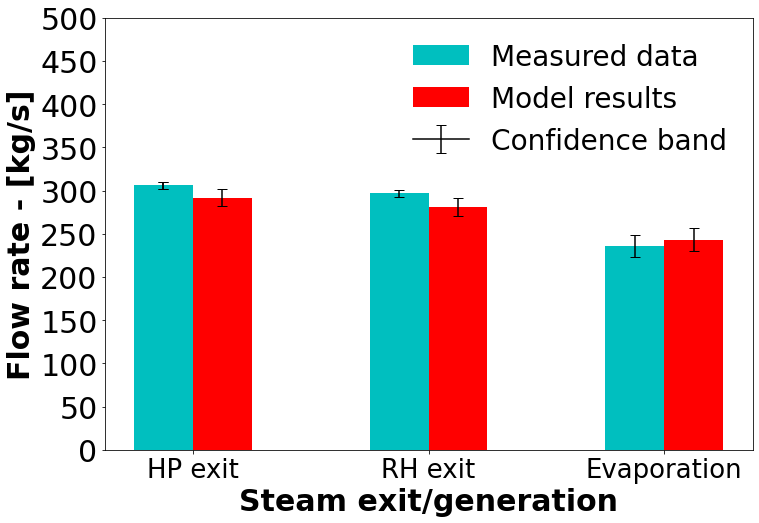
\includegraphics[width=\linewidth, height = 4.25cm]{60_CASE_STEAM}
    \caption{60\% MCR}
\end{subfigure}
\caption{Load validation result comparison of the measured data and MDN model results for the steam exit and  steam generation flowrates}
\label{fig_steam_gen}
\end{figure}

Considering the steam generation and exit flow rates of Figure \ref{fig_steam_gen} (a-c), the integrated model is shown to
sufficiently capture the hydraulic response of the case study boiler for a wide range of loads. A maximum under prediction of 8\% is found in the RH exit of the 60\% MCR load, and an over prediction of 4\% is realised in the RH exit 
ow rate of the 100\% MCR load. More uncertainty is associated with the integrated model, but this is deemed acceptable since the response overlaps with the measured data in all but one case, namely the 60\% MCR cases high-pressure and RH exit flow rates.\\

The attemperators of a utility scale boiler are an integral part of the control systems put in place to ensure safe operating conditions and minimal wear on the downstream components, namely the steam high-pressure and low-pressure steam turbines \cite{Kakac1991}. Figure  \ref{fig_attemp} (a-c) highlight the attemperator flow rates for the various MCR load cases. The results of ATT1
show that the integrated model can capture the attemperator flow rate entering between SH1 and SH2 with adequate accuracy, however the 80\% MCR load tends to over predict the mean ATT1 flow rate by 8\%. Furthermore, the ATT1 flow rates demonstrate the largest uncertainty of the integrated model results, which all overlap with the measured data confidence bands. The attemperator ATT2 flow rates are adequately resolved for the MCR loads, with a maximum over prediction of 8\%. The attemperator ATT-RH, demonstrates sufficiently accurate results across all validation MCR loads.\\
\begin{figure}[h!]
\centering
\begin{subfigure}{0.33\textwidth}
    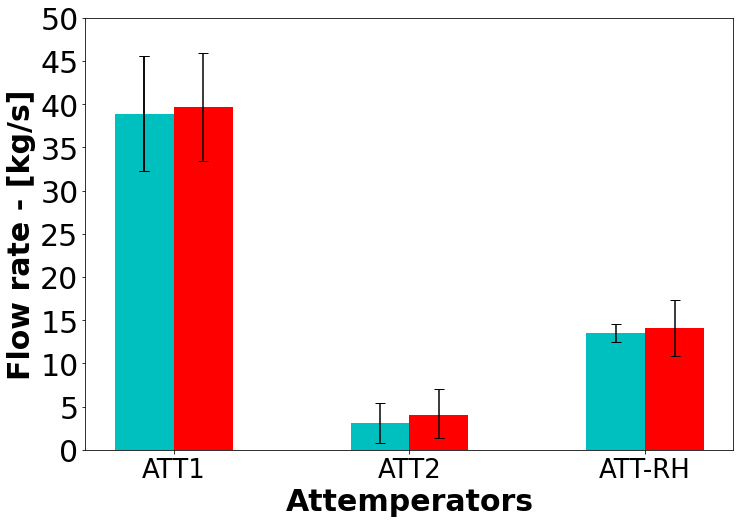
\includegraphics[width=\linewidth, height = 4.25cm]{100_CASE_ATTEMP}
    \caption{100\% MCR}
\end{subfigure}\hfill % maximize horizontal separation
\begin{subfigure}{0.33\textwidth}
    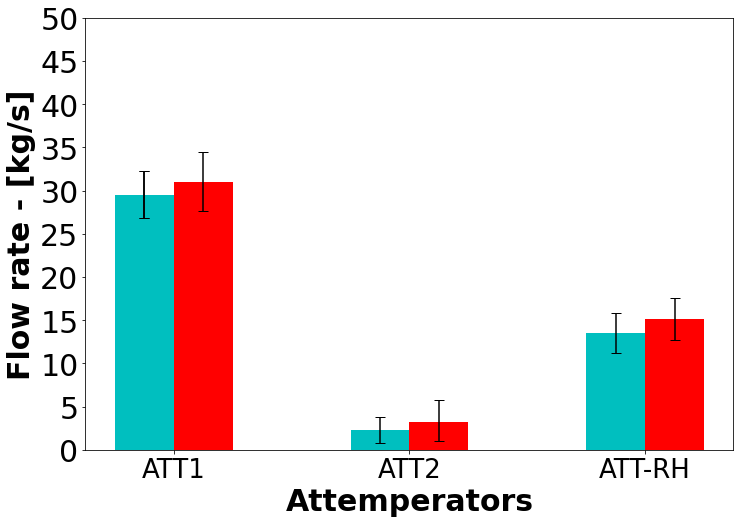
\includegraphics[width=\linewidth, height = 4.25cm]{80_CASE_ATTEMP}
    \caption{80\% MCR}
\end{subfigure}\hfill
\begin{subfigure}{0.33\textwidth}
    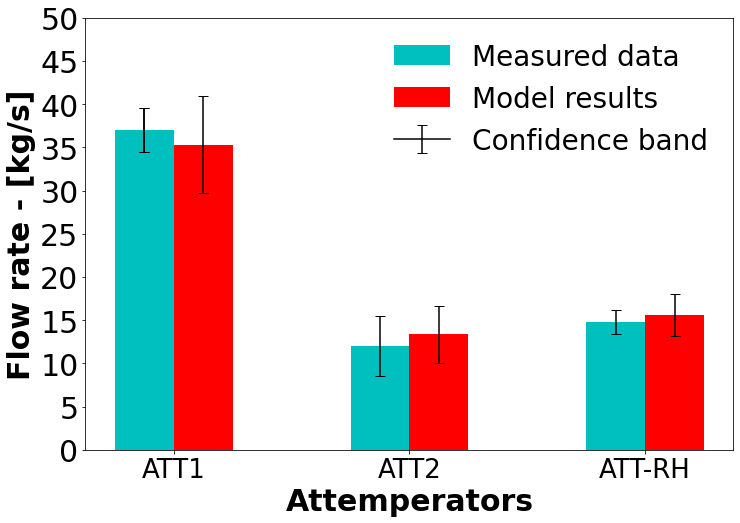
\includegraphics[width=\linewidth, height = 4.25cm]{60_CASE_ATTEMP}
    \caption{60\% MCR}
\end{subfigure}
\caption{Load validation result comparison of the measured data and MDN model results for the required attemperator flowrates to maintain operational integrity}
\label{fig_attemp}
\end{figure}

It has been shown that the integrated model is able to resolve the thermal response based on the predictions of the MDN model for a wide range of loads with sufficient accuracy. The heat loads are within a 10\% tolerance of the measured mean values, while the steam generation rates exhibit a maximum difference of 8\%, which is seen in the 60\% MCR load case (refer to Figure \ref{fig_steam_gen} (c)). The attemperator flow rate results show the largest uncertainty/confidence band of all the results (Figure \ref{fig_attemp}), however these overlap with the measured values. 
\subsection{Off-design analysis using the integrated model}
This section demonstrates the application of the validated integrated model by investigating the impact of fuel quality on the overall plant performance. The fuel quality parameters that are varied are the ash ($Y_{ASH}$) and moisture ($Y_{H_{2}O}$) contents, which in turn affect the HHV value of the respective fuel. Two case studies are considered, one where the ash content is significantly increased, and a second case whereby the moisture content is only increased. The boiler efficiency, heat pick-up and thermal response are investigated to determine the impact these abnormal off-design conditions can have on the boiler's performance. The input vectors for the two fuel cases are provided in Table \ref{tbl_inputs}. The inputs are the same as those of the 100\% load case except for the ash, moisture, and higher heating value of the respective fuels.\\

As with the validation case studies of Section \ref{sec_result_1}, the Monte Carlo method was employed to ascertain the mean and standard deviation values predicted via the integrated model. The base case in Figure \ref{fig_fuel_results} (a-c) refers to 100\% load case of Figures \ref{fig_heat_load}-\ref{fig_attemp}.\\
\begin{figure}[h!]
\centering
\begin{subfigure}{0.33\textwidth}
    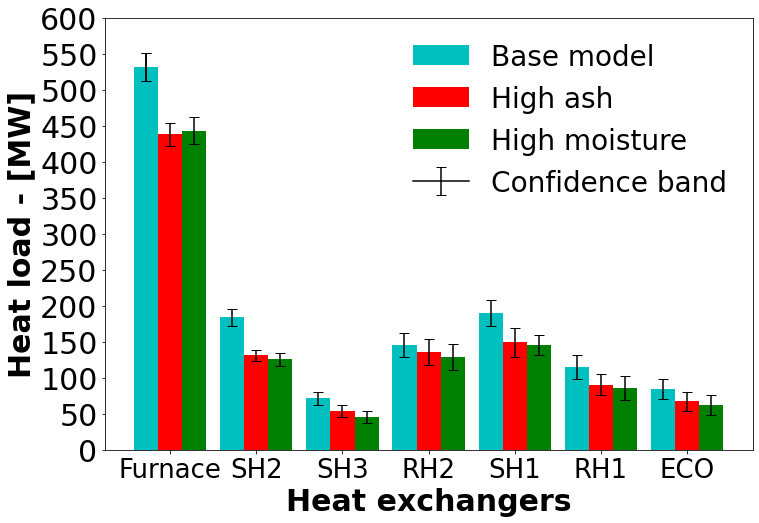
\includegraphics[width=\textwidth, height = 4.25cm]{100_FUEL_CASE}
    \caption{}
\end{subfigure}\hfill % maximize horizontal separation
\begin{subfigure}{0.33\textwidth}
    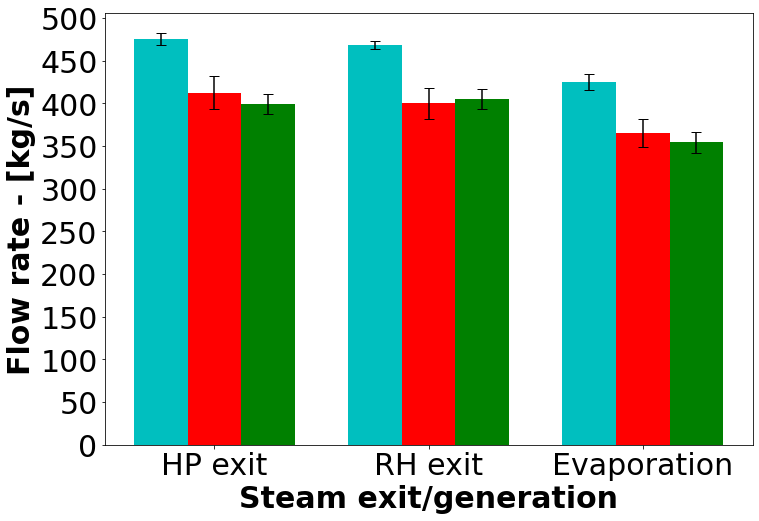
\includegraphics[width=\linewidth, height = 4.25cm]{100_FUEL_CASE_STEAM}
    \caption{}
\end{subfigure}\hfill
\begin{subfigure}{0.33\textwidth}
    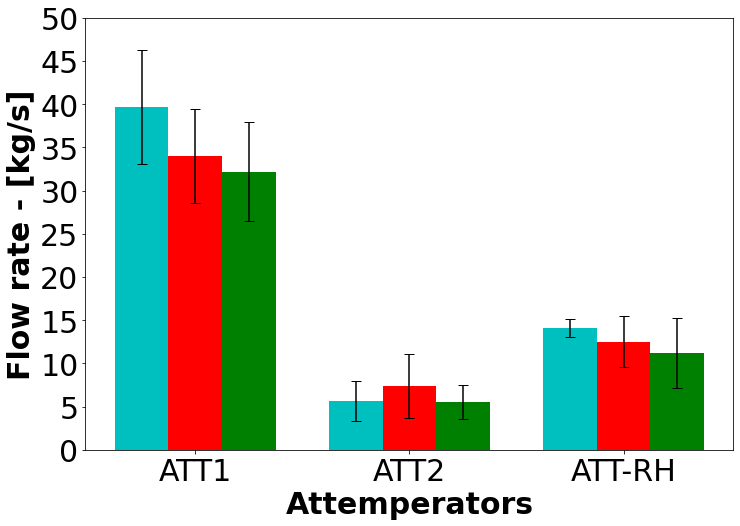
\includegraphics[width=\linewidth, height = 4.25cm]{100_FUEL_CASE_ATTEMP}
    \caption{}
\end{subfigure}
\caption{Integrated base case, high-ash and high-moisture case study comparison for; (a) the various heat exchangers, (b) the steam exit and generation flowrates, and (c) the required attemperator flowrates to maintain operational integrity}
\label{fig_fuel_results}
\end{figure}

Figure \ref{fig_fuel_results}  (a) highlights the effects that poor quality fuel has on the heat load to the various heat exchangers, with a 20\% drop being observed on average. This can reasonably be expected since the energy content of the fuel is lower than that of the base case. To maintain 100\% load capabilities using the poor quality fuel would require an increase in the fuel flow rate, which would provide more energy content. However, the mill operational capacities are limited. The operational protocol for the 100\% load case makes use of 5 mills operating 30 of the 36 burners at full capacity, with a standby mill and burner arrangement placed in reserve to help mitigate operational risks, such as maintenance schedules. Using the standby mill would allow the fuel flow rate to be increased by a maximum of 17\%. However, this would in turn decrease the operational integrity and increase the associated risks. This situation would therefore imply an unwanted load loss. When burning the high-ash content fuel the likelihood of ash deposition/fouling of the heat exchanger components also increases.\\
\newpage
Figure \ref{fig_fuel_results} (b-c) similarly illustrate a decrease in the water/steam flow rates for the steam exit and attemperator conditions. The generation rates exhibit similar characteristics to the 80\% load case of Figure \ref{fig_steam_gen} (b), illustrating a significant decrease in the operational capabilities when using a poor quality fuel. The predicted flue gas temperatures entering the convective pass are shown in Table \ref{tbl_fuel_results}. It is shown that for an increase in the ash content of the fuel, the flue gas inlet temperature increases, which results in a higher radiative heat transfer percentage for the convective pass components. It is also interesting to note that a higher ash content results in the largest uncertainties in the prediction of the high-pressure and RH exit steam and steam generation flow rates. The presence of more moisture in the fuel results in a lower inlet temperature, primarily since the extra moisture requires a higher heat rate of evaporation, leading to lower radiative heat transfer percentages.\\

The boiler efficiency is the measure used to convey how well the combustion heat is transferred to the working fluid and is defined as the ratio of total amount of heat absorbed by the heat exchangers (i.e. sum of the furnace, radiative and convective pass heat loads) and the combustion energy released ($\dot{m}_{fuel}HHV$). A significant decrease in the boiler efficiency is highlighted in Table \ref{tbl_fuel_results} for both fuel cases with the high ash fuel showing a slightly better result. The higher efficiency of the high-ash fuel is attributed to the fact that in general the heat loads to various heat exchangers are higher than that of the high-moisture fuel, which can be seen in Figure \ref{fig_fuel_results} (a). 

\begin{table}[pos=h]
\caption{Model results for poor quality fuel characteristics}\label{tbl_fuel_results}
\begin{tabular*}{\tblwidth}{p{0.3\textwidth}p{0.22\textwidth}p{0.22\textwidth}p{0.22\textwidth}}
\toprule
\textit{Variable} (\textbf{mean}  (\textit{min},\textit{max}))& Base & High-ash & High-moisture \\ % Table header row
\midrule
Mean boiler efficiency [\%]& \textbf{88.2}  (\textit{75.6},\textit{91.2}) & \textbf{77.6}  (\textit{73.4},\textit{80.9}) & \textbf{75.9}  (\textit{69.8},\textit{78.3})\\
Convective pass inlet flue gas temp. [$K$]& \textbf{1352}  (\textit{1339},\textit{1370}) & \textbf{1368}  (\textit{1354},\textit{1378}) & \textbf{1311}  (\textit{1295},\textit{1327})\\
\midrule
\multicolumn{4}{l}{\textit{Radiative heat transfer percentage (Convective pass)} }\\
\midrule
RH2 & \textbf{52.3}  (\textit{50.1},\textit{54.0}& \textbf{56.2}  (\textit{52.9},\textit{58.5} & \textbf{50.3}  (\textit{47.8},\textit{53.9}\\
SH1 & \textbf{46.3}  (\textit{43.0},\textit{49.2})& \textbf{49.8}  (\textit{44.8},\textit{52.3}& \textbf{47.2} - (\textit{43.2},\textit{50.8}\\
RH1 & \textbf{21.3}  (\textit{16.1},\textit{24.6})& \textbf{26.7}  (\textit{20.6},\textit{30.1}& \textbf{18.2}  (\textit{13.7},\textit{23.5}\\
ECO & \textbf{6.7}  (\textit{5.1},\textit{9.8})& \textbf{8.3}  (\textit{6.3},\textit{12.6}& \textbf{5.4} - (\textit{2.8},\textit{9.7}\\
\bottomrule
\end{tabular*}
\end{table}  
\newpage
\section{Conclusion}
The present work establishes the basis for utilising an integrated data-driven surrogate and 1-D process model to investigate the overall operational response for a 620 [$MW_e$] utility scale boiler.\\

The data-driven surrogate modelling approach using CFD simulations can predict the various parameters needed to capture the combustion and heat transfer characteristics. These include the heat loads to the furnace evaporator walls (EV) and radiative superheaters (SH2 and SH3), as well as the flue gas characteristics entering the convective pass, which include the temperatures, species mass fractions and radiation intensity. Training and testing datasets were generated using the CFD model of the 620 [$MW_e$]. A total of 180 different CFD simulation cases were performed, where the input variables of Table \ref{tbl_doe} were varied.\\

It was found that the best surrogate model architecture was the use of a MDN configuration, which also allows prediction of the associated uncertainties. The configuration comprised of a MDN network consisting of 4 hidden layers each consisting of 80 neurons and 3 normal output distributions, while using a learning rate of $1\times10^{-5}$ and batch size of 32. The MDN network illustrated that approximately 80-85\% of the model predictions had MAPEs below 10\%.\\

A validation case study was performed using the integrated model for a wide range of operational loads. The model results were compared to the measured thermal response for all load cases. The resolution of the heat loads, steam flow rates and attemperation flow rates resulted in a maximum difference of 7\%. The uncertainties predicted by the surrogate model were propagated through the integrated model using the Monte Carlo technique, adding valuable insight into the operational limits of the power plant and the uncertainties associated with it.\\

The application case studies considered the impact of poor quality fuels at 100\% MCR operation. The results highlight the drop in performance due to the fuel quality resulting in a substantial decrease in boiler efficiency. Using a high-ash fuel can result in a higher exit flue gas temperatures resulting in a marginal increase in performance of the convective pass heat exchangers when compared to the high moisture fuel. However, it results in greater uncertainty in the predicted steam exit and generation flow rates and increases the likelihood of ash deposition occurring.\\ 

The current work has shown that it is possible to adequately resolve the thermofluid response of a utility scale boiler using a data-driven surrogate model trained on CFD simulation results. The integration of the surrogate and 1-D process model is paramount in modelling the thermal response and provides valuable operational insight for various load cases, including the uncertainty in the predicted results. The methodology used in the present work can be applied by engineers and other researchers to investigate various effects on the whole boiler operation.
\section*{Acknowledgements}
The authors would like to thank the Centre for High Performance Computing (CHPC) in South Africa for providing computational resources.

\printcredits
%% Loading bibliography style file
%\bibliographystyle{model1-num-names}
%\bibliographystyle{cas-model2-names}
\bibliographystyle{elsarticle-num}

% Loading bibliography database
\bibliography{ML_paper}

%\begin{flalign} \label{eqn_cfd}
%&\frac{\partial}{\partial x_{i}}(\rho \bar{u}_{i})=S \nonumber &&\\
%&\frac{\partial}{\partial x_{i}}(\rho_{eff} u_{i}u_{j})+\frac{\partial %\overline{p}}{\partial x_{j}} = \frac{\partial}{\partial x_{i}}\left[\mu\left\%{\frac{\partial u_{j}}{\partial x_{i}}+\frac{\partial u_{i}}{\partial x_{j}}-%\frac{2}{3}\delta_{ij}\frac{\partial u_{i}}{\partial x_{i}}\right\}\right]+%\frac{\partial}{\partial x_{i}}(-\rho\overline{u_{i}^{'}u_{j}^{'}})+S_m %\nonumber &&\\
%&\frac{\partial }{\partial x_{i}} (u_{i}[\rho E+p])=\frac{\partial }{\partial %x_{j}}\left[\lambda\frac{\partial T_{g}}{\partial x_{j}}\right] +S_{h} &&\\
%&\frac{\partial}{\partial x_{i}}(\rho u_{j}Y_{k})=-\frac{\partial}{\partial %x_{j}}(\vec{J_{k}})+ \sum_r R_{j,r} + S_{k} \nonumber && 
%\end{flalign}
\end{document}


